% !TeX root = index.tex
% define document class
\documentclass{scrreprt}

% set variables
\newcommand{\varAuthor}{Anes Hodza}
\newcommand{\varCandidate}{\textbf{\varAuthor} \\ anes.hodza04@gmail.com} % Kandidat/in
\newcommand{\varResponsibleSpecialist}{\textbf{Josua Schmid} \\ josua.schmid@renuo.ch} % verantwortliche Fachkraft
\newcommand{\varVocationalTrainer}{\textbf{Sophie Nemet} \\ sophie.nemet@kbw.ch} % Berufsbildner/in
\newcommand{\varPrimaryExpert}{\textbf{Touseef Arif} \\ touseef.arif@aliff.ch} % Hauptexperte
\newcommand{\varSecondaryExpert}{\textbf{Kevin Cina} \\ pk19@cinas.ch} % Nebenexperte
\newcommand{\varCompany}{Renuo AG} % Firmenname
\newcommand{\varCompanyDepartment}{Entwicklung} % Abteilungsname
\newcommand{\varTitle}{Redmine Plugin: Entwicklungsstand}
\newcommand{\varVersion}{0.2} % Versionsnummer: Pro IPA-Tag um 0.1 erhöhen
\newcommand{\varExaminationBoard}{Prüfungskomission 19} % Prüfungsorganisation
\newcommand{\varExaminationBoardDepartment}{Informatik Applikationsentwicklung} % Fachrichtung

% apply ipa package
\usepackage{../lib/ipa}
\usepackage{../lib/tikz-uml}

% own packages
\usepackage{soul}

\lohead[\varTitle]{\varTitle}
\lofoot[\today]{\today}
% see B6.5
\cfoot[\varAuthor\ / \varCompany\\Version \varVersion]{\varAuthor\ / \varCompany\\Version \varVersion}
\rofoot[Seite \pagemark{} von \pageref{LastPage}]{Seite \pagemark{} von \pageref{LastPage}}

% load sources
\addbibresource{sources.bib}

% make glossaries
\makenoidxglossaries

% define glossary entries
\newglossaryentry{Redmine}{
  name={Redmine},
  description={Redmine ist ein Open-Source Projektmanagement-Tool. Es basiert auf Ruby on Rails und erlaubt das
  erstellen von Plugins.}
}

\newglossaryentry{Linter}{
  name={Linter},
  description={Ein Linter ist ein Programm, welches Quell-Code auf Fehler, wahrscheinliche Bugs und Stilfehler überprüft.}
}

\newglossaryentry{Ticket}{
  name={Ticket},
  description={Ein Ticket (im Kontxt dieser PA) ist eine Aufgabe, welche im Redmine System eingetragen ist. Diese kann
  ein Feature-Request, ein Bug oder eine andere Aufgabe sein.}
}

\newglossaryentry{Redmine-Ticket}{
  name={Redmine Ticket},
  description={Ein \enquote{Redmine-Ticket} ist ein Ticket. Im Rahmen dieser PA werden beide Begriffe synonym
  verwendet.}
}

\newglossaryentry{Issue}{
  name={Issue},
  description={Ein Issue ist das von Redmine offiziell verwendete Wort für ein Ticket. Im Rahmen dieser PA werden
  beide Begriffe synonym verwendet.}
}


% create document
\begin{document}

  % set page numbering
  \pagenumbering{roman}

  % set page style
  \pagestyle{scrheadings}

  % include title page
  \thispagestyle{empty}
  
  \begin{center}
  \makebox[\textwidth]{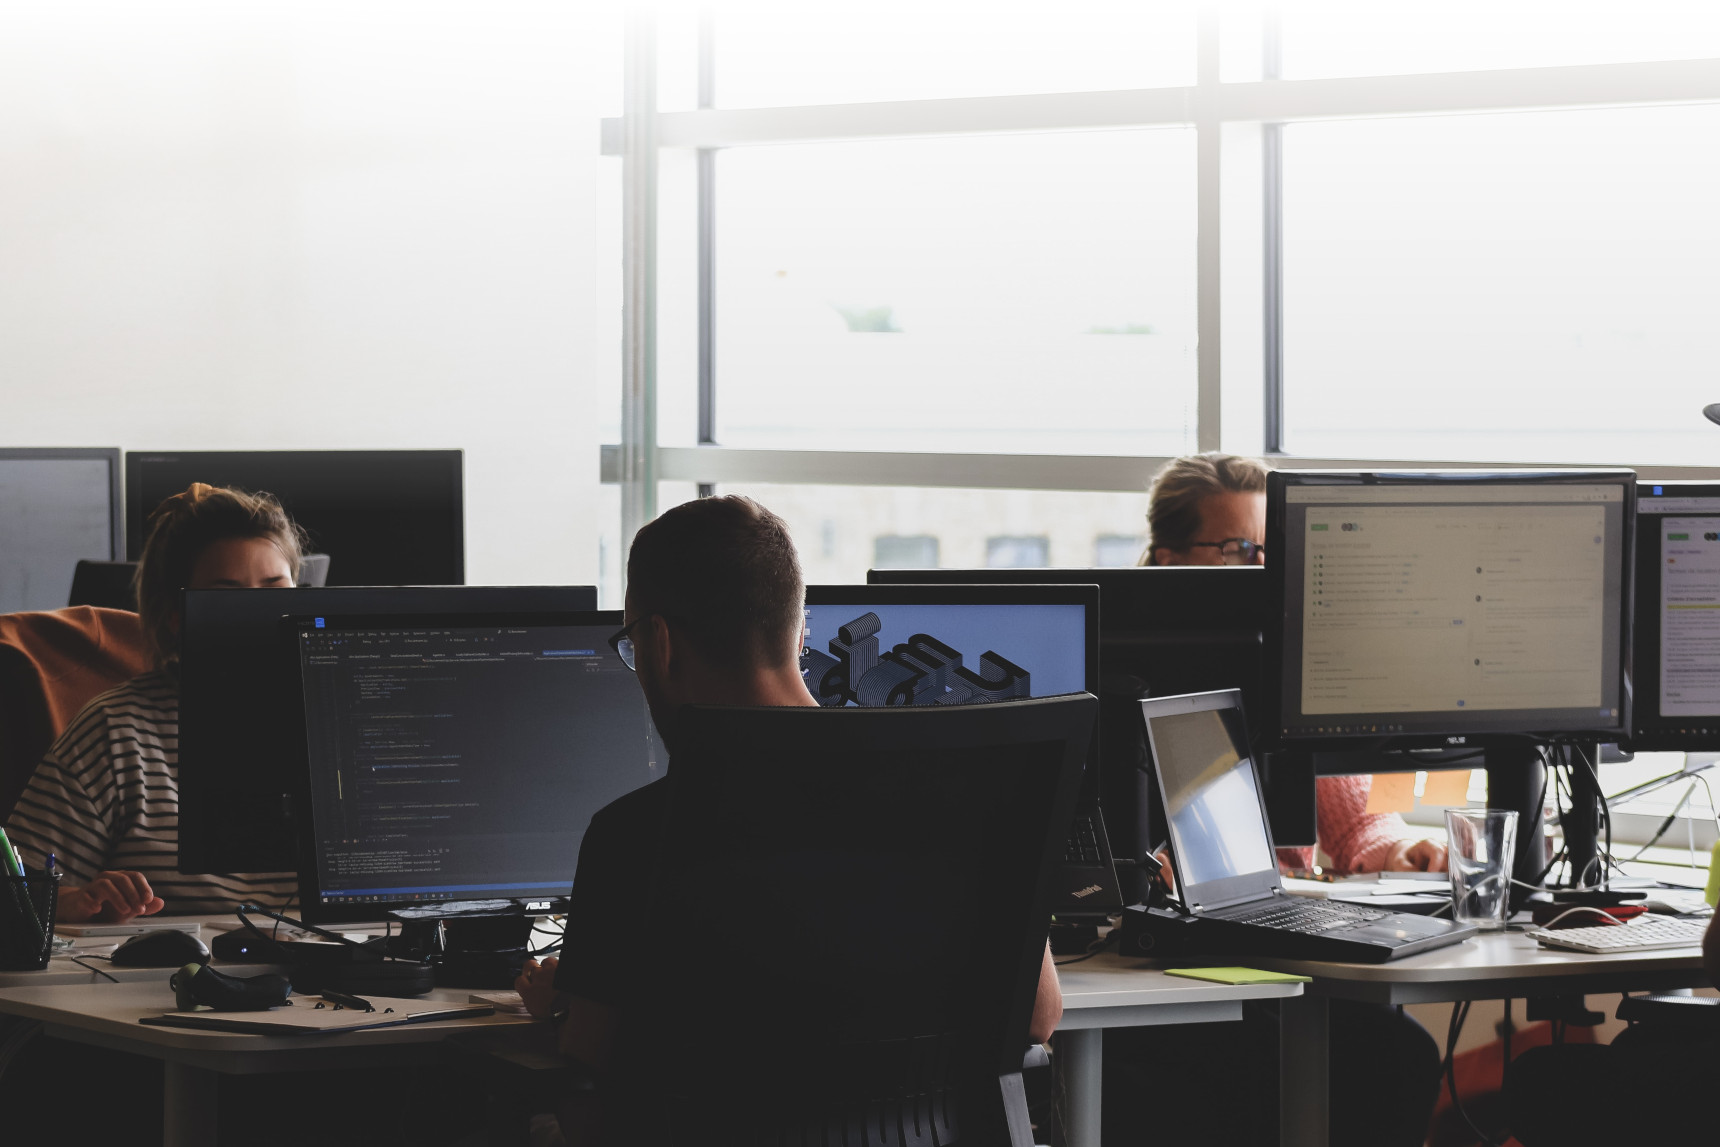
\includegraphics[width=1.1\paperwidth]{images/title.jpg}}
\end{center}
\vspace*{1cm}
{\fontsize{28}{28}\selectfont \varTitle}\\[0.25cm]
{\fontsize{16}{16}\selectfont \varAuthor}\\[0.25cm]
{\fontsize{16}{16}\selectfont \varCompany}

  \newpage
  \TileWallPaper{\paperwidth}{\paperheight}{images/background.pdf}

  % see A1.3
  % see B6.3
  % generate the table of contents
  \tableofcontents

  % finish page
  \clearpage

  % use the arabic numbering system
  \pagenumbering{arabic}

  % reset page counter
  \setcounter{page}{1}

  % see B6.1a
  % create a phantom toc entry for "Umfeld und Ablauf"
  \clearpage\phantomsection\addcontentsline{toc}{part}{Umfeld und Ablauf}

  % [2]: Seite 11
\chapter{Aufgabenstellung}

Dieses Kapitel beinhaltet die komplette Aufgabenstellung im originalen Wortlaut.

\section{Ausgangslage}

Die Renuo AG verwendet Redmine, eine freie, webbasierte Projektmanagement-Software. Alle Kundenprojekte und internen Aufgaben werden in Redmine mithilfe von Tickets orchestriert. Ein Product-Owner (PO) erarbeitet die Anforderungen zusammen mit dem Kunden, schreibt sie in das Ticket und übergibt sie an die Entwickler. Danach startet die Implementationsphase. Diese Phase durchläuft je nach Grösse des Projektes verschiedene Ticket-Status (\enquote{in progress}, \enquote{in review}, \enquote{on staging}, \enquote{to deploy}, \enquote{on master}). In dieser Zeit muss sich der PO darauf verlassen, dass der zuständige Entwickler den Ticket-Status gewissenhaft nachführt. Das ist aber oft nicht repräsentativ für den wirklichen Entwicklungsstand. Es passiert immer wieder, dass Code-Reviews oder das Testen auf dem Staging-Server durch den Kunden lange dauern. Der PO muss sich also immer wieder bei den Entwicklern nach dem Stand der Tickets erkundigen. Da wir mit Git-Feature-Branches arbeiten, wäre eigentlich die Redmine-Ticketnummer in unseren Git-Branches verfügbar.

Das Ziel dieser Arbeit ist es, die Arbeit des PO zu vereinfachen. Dazu wird ein Redmine-Plugin entwickelt, das im Ticket die zugehörigen GitHub-Pull-Requests und Semaphore-Deployments anzeigt. Als Identifikation der Code-Zugehörigkeit wird die Redmine-Ticketnummer im Git-Branch verwendet.

\section{Detaillierte Aufgabenstellung}

Die Software bedient folgende Benutzerrolle: \newline
- \enquote{PO} (Product-Owner) spezifiziert und kontrolliert Redmine-Tickets. \newline
- \enquote{Entwickler} implementiert Source-Code anhand eines Redmine-Tickets. \newline

Folgende User-Stories sollen verwirklicht werden: \newline
- F1: Als PO möchte ich alle zum Ticket zugehörigen GitHub-Pull-Requests in einer Liste sehen, damit ich den Entwicklungsfortschritt des Tickets beurteilen kann. Die Listeneinträge enthalten den Status der Pull-Requests (draft, open, merged) und sind klickbare Links, die direkt zu GitHub abspringen (z.B. \url{https://github.com/renuo/rails\_api\_logger/pull/3}). Die Identifikation des zugehörigen Pull-Requests findet über die Ticketnummer im Branch-Namen statt. \newline
- F2: Als PO möchte ich eine Liste der Semaphore-Deployments zum Ticket sehen. Ich sehe das Datum und den Status (Erfolg, Misserfolg). Jeder Listeneintrag ist ein klickbarer Link, der zu Semaphore abspringt. Der Status kann auch einfach farbcodiert sein. \newline
Anzuzeigen sind Deployments von den develop und master/main-Git-Branches. \newline
Achtung: Es kann nicht einfach so auf einen Branch-Namen eines gelöschten Branches geschlossen werden. Zur Identifikation des Redmine-Tickets soll die Pull-Request-Nummer aus der von Semaphore zurückgegebenen commit\_message verwendet werden um über den GitHub-Pull-Request Rückschlüsse zu ziehen (via GitHub-API). \newline
Es gelten folgende nicht-funktionalen Anforderungen: \newline
- Software-Design: Das Plugin muss so entkoppelt von Redmine sein, wie möglich. So sollen z.B. bestehende Redmine-Tabellen nicht verändert werden (Join-Tables verwenden). \newline
- Software-Design: Das Plugin soll sich an die Coding-Guidelines von Redmine halten und schon vorhandene Bibliotheken nutzen (z.B. Minitest, ERB statt Slim). \newline
- Software-Design: Die Informationen zum externen Fortschritt müssen beim Öffnen der Ticket-Ansicht schon verfügbar sein. Etwaige Synchronisierung soll mittels Background-Job oder im Webhook-Call umgesetzt werden. \newline
- Software-Design: Die zwei Aspekte Pull-Request und Deployment-Status sollen möglichst voneinander getrennt werden. GitHub und Semaphore sollten beide in Zukunft austauschbar sein. \newline
- Software-Design: Das Plugin soll auf Webhooks von GitHub und Semaphore hören. Aktives Polling beider Services sollte vermieden oder zumindest sehr gut begründet werden. \newline
- Sicherheit: Webhooks von GitHub und Semaphore ermöglichen einen sparsamen Umgang mit API-Zugängen. Zum Beispiel sollte das zu entwickelnde Plugin für die Semaphore-Status-Anzeige auf schon geschehene Webhook-Calls von GitHub zurückgreifen, statt explizit selbst nochmals GitHub aufzurufen. Falls das nicht immer geht, dürfen zur Verbesserung der Sicherheit begründete Kompromisse beim Feature-Umfang eingegangen werden. \newline
- UX: Für die Bedienung darf kein dediziertes Benutzerhandbuch notwendig sein. \newline
- Dokumentation: Wichtige Teile der Software müssen mit den richtigen UML-Diagrammen beschrieben werden: \newline 
 - Entity-Relationship-Diagramm für die Business-Domain \newline
 - Activity-Diagramm für die Synchronisierung des externen Fortschritts \newline
- Dokumentation: Die Funktionsweise des Plugins muss im README des Projektes kurz aufgezeigt werden. \newline
- Tests: Der Happy-Path muss automatisiert End-to-end getestet sein (System-Tests). \newline
- Tests: Die Unit-Test-Abdeckung des Plugins beträgt 100\%. \newline
- Tests: Zugriffe auf die GitHubl und die Semaphore-API müssen in den Tests gemockt werden. \newline

\section{Mittel und Methoden}
Für die IPA werden folgende Technologien eingesetzt: \newline
- Redmine 4.x und 5.x (Plugin-Kompatibilität) \newline
- Ruby on Rails 5.2 bis 7.0 (Plugin-Kompatibilität) \newline
- MiniTest und Capybara \newline
- Rubocop \newline
- HTML5 (HTML, JS, CSS) \newline
- Postgres \newline

Die zu entwickelnde Software läuft auf dem Macbook des Kandidaten mit einem aktuellen Chrome-Browser. \newline

  % [2]: Seite 11
\chapter{Deklaration}

Folgender Abschnitt beschreibt die Vorkenntnisse des Kandidaten und dessen Vorbereitung.

\section{Vorkenntnisse}

\lipsum[11]

\section{Vorarbeiten}

\lipsum[12]

\section{Neue Lerninhalte}

\lipsum[13]

\section{Arbeiten in den letzten 6 Monaten}

\lipsum[14]

  \chapter{Arbeitsumfeld}

\section{Firmenstandards}
Die Renuo AG verwendet verschiedene Tools zur Garantie der Codequalität. Diese Tools werden in diesem Kapitel dokumentiert.
\subsection{Code-Analyse}
Für sauberes Formatieren werden je nach Sprache unterschiedliche \gls{Linter} verwendet. Nebenbei können auch andere Tools, welche die Sicherheit verbessern, genutzt werden. In diesem Falle werden folgende Tools verwendet:
\begin{itemize}
    \item \textbf{Rubocop} wird für Ruby Quellcode verwendet.
    \item \textbf{Brakeman} wird für das Vermeiden von groben Sicherheitslücken verwendet.
\end{itemize}
\subsection{Tests}
Um die Funktionalität des Programmes zu garantieren, werden automatisierte Tests geschrieben. Dabei soll jede einzelne Zeile (falls die Klasse über fünf Zeilen hat) getestet werden.
\subsection{Code Review}
Um die Qualität des Codes zu garantieren, wird dieser von einem anderen Entwickler überprüft. Da dieses Projekt eine Einzelarbeit ist, wird der Quellcode vom Kandidaten selber überprüft.

\section{Entwicklungsumgebung}
\subsection{Versionierung}
Für die Versionierung wird Git verwendet. Dabei wird GitHub als Remote-Repository verwendet. Das Repository mit
dem Source-Code kann unter \url{https://github.com/aneshodza/gnosis} gefunden werden. Für eine genauere Beschreibung
der Versionierung siehe Kapitel \ref{sec:versioning}.
\subsection{IDE}
Als IDE wird vim mit verschiedenen Plugins verwendet. Bestimmte Sachen wurden in der \bgmintinline{bash}{.vimrc} Datei
konfiguriert, damit die Arbeit möglichst effizient ist. \newline
Diese Konfigurationen sind unter \newline
\url{https://github.com/aneshodza/.dotfiles/blob/ad87ee9ecc5588a59d66e211797792099569ca95/.vimrc} zu finden.
\subsection{CI/CD}
Für die CI/CD Pipeline wird SemaphoreCI verwendet. Das ist passend, da auch die PA sehr eng mit SemaphoreCI verbunden
ist.

  % see B6.2a
\chapter{Projektaufbauorganisation}

% Diesen Abschnitt anpassen.
Das Projekt \placeholder\ wird in der Abteiltung \enquote{\varCompanyDepartment} umgesetzt. Projektleiter ist \placeholder\ und für die IPA auch die verantwortliche Fachkraft. Für die fachliche Umsetzung des hier beschriebenen Projekts ist ausschliesslich die Zusammenarbeit zwischen \placeholder\ und dem Kandidaten notwendig.

Im Unterschied zur üblichen Arbeit im Betrieb, werden zwei Experten die Arbeits des Kandidaten Begleiten und Bewerten. Die Projektaufbauorganisation ist in \ref{fig:organigram} visualisiert.

\begin{figure}[H]
  \begin{multicols}{2}
    \begin{forest}
      for tree={draw,grow'=0,folder,align=left}
      [\textbf{\varCompany}
        [\textbf{HR}
          [(BB) \\ \varVocationalTrainer]
        ]
        [...]
        [\textbf{\varCompanyDepartment}
          [(VF) \\ \varResponsibleSpecialist]
          [(K) \\ \varCandidate]
        ]
      ]
    \end{forest}

    \begin{forest}
      for tree={draw,grow'=0,folder,align=left}
      [\textbf{\varExaminationBoard}
        [\textbf{\varExaminationBoardDepartment}
          [(HEX) \\ \varPrimaryExpert]
          [(NEX) \\ \varSecondaryExpert]
        ]
      ]
    \end{forest}
  \end{multicols}
  \caption[\enquote{Organigramm der am Projekt teilnehmenden Personen} visualisiert mit TikZ Forest]{\gls{Organigramm} der am Projekt teilnehmenden Personen}
  \label{fig:organigram}
\end{figure}
  % see A1.2
% see A3
% see B6.2b
\begin{landscape}
  \chapter{Zeitplan}
  Der Zeitplan basiert auf der Vorlage \cite{Buhler_ipa-timetable_2022} und zeigt mit einer Auflösung von zwei Stundenblöcken die geplanten und getätigten Aufwände.
  \begin{figure}[H]
    \begin{center}
      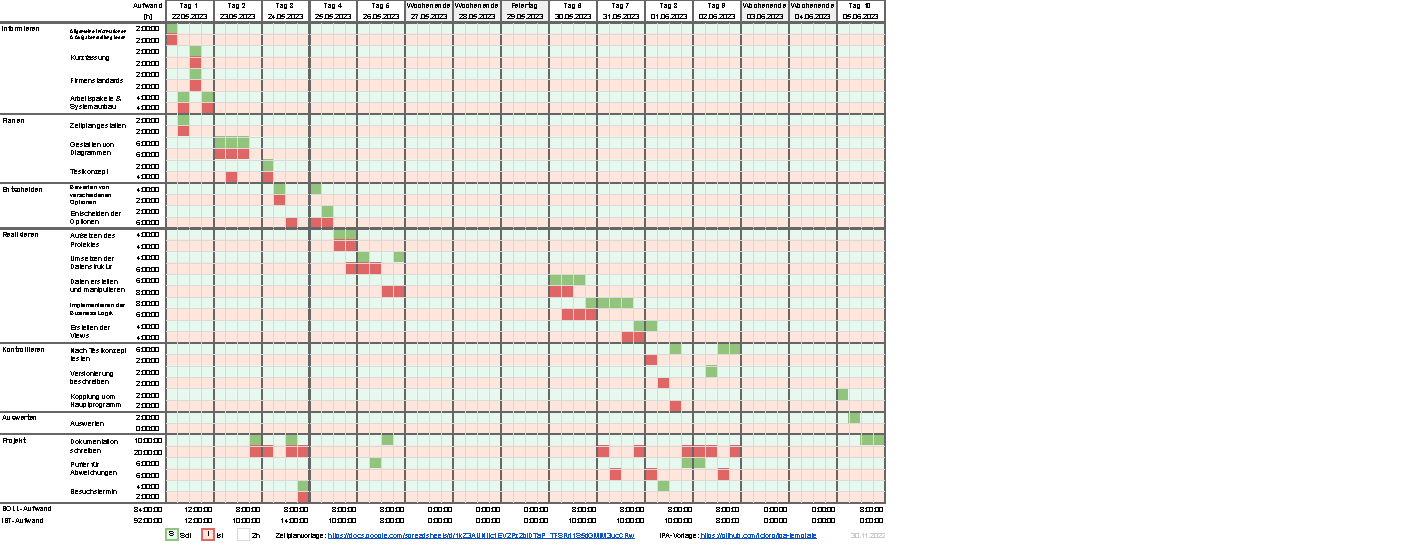
\includegraphics[width=1.55\textheight]{../res/timeplan.pdf}
    \end{center}
    \caption[\enquote{Zeitplan} erstellt mit Google Sheets]{Zeitplan}
    \label{fig:timeplan}
  \end{figure}
\end{landscape}

  \chapter{Expertengespräche}
\section{Erstes Expertengespräch}
\label{sec:first-expert-meeting}
Das erste Expertengespräch fand am \textbf{24. Mai 2023 um 17:30} statt. Es war ein remote Meeting auf Zoom.
Die Teilnehmer waren:
\begin{itemize}
  \item \textbf{Anes Hodza} (Kandidat)
  \item \textbf{Touseef Arif} (HEX)
\end{itemize}

\subsection{Ablauf des Meetings}
Zu Beginn stellten sich beide Teilnehmer vor. Anschliessend bat der HEX den Kandidaten darum, die Aufgabenstellung
zusammenzufassen. Der Kandidat erklärte, dass er ein Redmine Plugin erstellen soll, welches \gls{Issue}s mit Pull Requests
sowie Deployments verknüpft. Der HEX bestätige dies. \newline
Danach ging der HEX mit dem Kandidaten die Persönlichen Anforderungen durch, um zu verifizieren, dass beide auf der
gleichen Seite sind. Dabei wurde auch klar, dass der Kandidat die Anforderungen verstanden hat. \newline
Als Nächstes wurde geklärt, was der momentane Status bezüglich der VF ist. Diese ändert sich eventuell noch. \newline
Schlussendlich erklärte der HEX dem Kandidaten welchen Inhalt der Glossar haben soll: Firmeninterne Begriffe, welche
für aussenstehende nicht verständlich sind. Der Kandidat kann sich darauf verlassen, dass der HEX Fachbegriffe
versteht. \newline

\section{Zweites Expertengespräch}
\label{sec:second-expert-meeting}

  % see A2.1
% see B6.2c
\chapter{Arbeitsjournal}

\section{Tag 1}
\begin{tabularx}{\textwidth}[H]{|c|X|}
  \hline
  Gearbeitete Zeit & 8.92h \\ \hline
  Erledigte Arbeiten & Heute wurde die PA gestartet. Ich fing damit an, die Dokumentation anhand vom Template
  \cite{Buhler_ipa-template_2022} zu erstellen. Danach kümmerte ich mich um die allgemeinen Informationen und die
  Aufgabenstellung vom PkOrg. Von dort kopierte ich auch verschiedene Texte, wie zum Beispiel die
  Deklarationen (Kapitel \ref{chap:declaration}). \newline
  Dann wurde der Zeitplan mit den Arbeitspaketen erstellt, die Zusammenfassung der Aufgabe und die
  Firmenstandards.
  \\ \hline
  Ungeplante Arbeiten & Keine. \\ \hline
  Erfolge & Die Basis für die Dokumentation steht bereits und ich bin momentan perfekt auf dem Zeitplan. \newline
  Ausserdem komme ich massiv besser mit LaTeX zurecht, als ich erwartet habe.
  \\ \hline
  Misserfolge & Das Korrigieren von Rechtschreibfehlern geht länger als vorher geplant.  \\ \hline
  Hilfestellungen & Die LaTeX Dokumentation von Overleaf \cite{overleaf} war mir eine grosse
  Hilfe, da ich noch eher unbekannt bin mit LaTeX. \\
  \hline
\end{tabularx}

\newpage

\section{Tag 2}
\begin{tabularx}{\textwidth}[H]{|c|X|}
  \hline
  Gearbeitete Zeit & 8.50h \\ \hline
  Erledigte Arbeiten & Heute ging es primär darum die Diagramme unter Kapitel \ref{chap:plan}
  (Planen) zu erstellen. Daneben ging es noch ein bisschen darum, die Arbeit von gestern
  aufzuräumen. Einige Punkte wurden übersehen, wie zum Beispiel die Erklärung von zwei
  externen Schnittstellen. Zu Ende wurde allgemein an der Dokumentation gearbeitet, wie
  im Zeitplan eingetragen. \\ \hline
  Ungeplante Arbeiten & Unerwartet begann die Arbeit am Testkonzept bereits. Das passierte,
  da ich eine Frage an die VF hatte, aber diese am Vormittag nicht erreichbar war. Nachdem
  die Unklarheiten aus dem Web geräumt wurden, ging die Arbeit wie geplant weiter.
  \\ \hline
  Erfolge & Dank der Arbeit am Testkonzept konnte ich mir einen kleinen Vorsprung zum
  Zeitplan machen. Die gewonnene Zeit kann gut als Puffer beim Implementieren genutzt werden.
  \\ \hline
  Misserfolge & Heute gab es keine Misserfolge \\ \hline
  Hilfestellungen & Die VF erklärte mir Software-Design Anforderung 3: \enquote{Die 
  Informationen müssen beim öffnen der Ticket-Ansicht schon verfügbar sein}.  \\ \hline
\end{tabularx}

\newpage

\section{Tag 3}
\begin{tabularx}{\textwidth}[H]{|c|X|}
  \hline
  Erledigte Arbeiten & Der Tag begann damit, die Diagramme vom Vortag leicht auszubessern. Zu
  Beginn wurde das Activity Diagramm angepasst, da es nicht ganz realitätsgetreu war. Dann wurde
  noch ein Vorschlag für das ERD hinzu gefügt. Die ERD Anpassung ergab sich aus der Activity
  Anpassung \newline
  Danach wurde das Testkonzept finalisiert. Da Arbeit bereits am Vortag begonnen wurde, mussten
  nur die manuellen Testfälle noch erstellt werden. \newline
  Dann wurden wieder Änderungen an den Diagrammen vorgenommen. Als erstes wurde ein neues Mockup
  hinzugefügt, welches den dritten (neuen) Vorschlag für das ERD besser darstellt. Dank den neuen
  Informationen ergab sich auch, dass das geplante Activity Diagramm für die SemaphoreCI Webhook
  wahrscheinlich nicht umsetzbar ist, weshalb ein \enquote{Fallback Plan} erstellt wurde. \newline
  Dann wurde endlich am Bewerten gearbeitet. Dieses Kapitel wurde auch schon abgeschlossen, weshalb
  das Entscheiden schon zum Teil erledigt werden konnte. \newline
  Zum Schluss war der Expertenbesuch, welcher dokumentiert wurde. Da sich beim Meeting herausstellte,
  dass die Anforderung zum Glossar nicht ganz verstanden wurden, wurde diese nochmals angepasst.
  \\ \hline
  Ungeplante Arbeiten & \lipsum[24] \\ \hline
  Erfolge & \lipsum[25] \\ \hline
  Misserfolge & \lipsum[26] \\ \hline
  Hilfestellungen & \lipsum[27] \\
  \hline
\end{tabularx}

\newpage

\section{Tag 4}
\begin{tabularx}{\textwidth}[H]{|c|X|}
  \hline
  Erledigte Arbeiten & \lipsum[23] \\ \hline
  Ungeplante Arbeiten & \lipsum[24] \\ \hline
  Erfolge & \lipsum[25] \\ \hline
  Misserfolge & \lipsum[26] \\ \hline
  Hilfestellungen & \lipsum[27] \\
  \hline
\end{tabularx}

\newpage

\section{Tag 5}
\begin{tabularx}{\textwidth}[H]{|c|X|}
  \hline
  Erledigte Arbeiten & \lipsum[23] \\ \hline
  Ungeplante Arbeiten & \lipsum[24] \\ \hline
  Erfolge & \lipsum[25] \\ \hline
  Misserfolge & \lipsum[26] \\ \hline
  Hilfestellungen & \lipsum[27] \\
  \hline
\end{tabularx}

\newpage

\section{Tag 6}
\begin{tabularx}{\textwidth}[H]{|c|X|}
  \hline
  Erledigte Arbeiten & \lipsum[23] \\ \hline
  Ungeplante Arbeiten & \lipsum[24] \\ \hline
  Erfolge & \lipsum[25] \\ \hline
  Misserfolge & \lipsum[26] \\ \hline
  Hilfestellungen & \lipsum[27] \\
  \hline
\end{tabularx}

\newpage

\section{Tag 7}
\begin{tabularx}{\textwidth}[H]{|c|X|}
  \hline
  Erledigte Arbeiten & \lipsum[23] \\ \hline
  Ungeplante Arbeiten & \lipsum[24] \\ \hline
  Erfolge & \lipsum[25] \\ \hline
  Misserfolge & \lipsum[26] \\ \hline
  Hilfestellungen & \lipsum[27] \\
  \hline
\end{tabularx}

\newpage

\section{Tag 8}
\begin{tabularx}{\textwidth}[H]{|c|X|}
  \hline
  Erledigte Arbeiten & \lipsum[23] \\ \hline
  Ungeplante Arbeiten & \lipsum[24] \\ \hline
  Erfolge & \lipsum[25] \\ \hline
  Misserfolge & \lipsum[26] \\ \hline
  Hilfestellungen & \lipsum[27] \\
  \hline
\end{tabularx}

\newpage

\section{Tag 9}
\begin{tabularx}{\textwidth}[H]{|c|X|}
  \hline
  Erledigte Arbeiten & \lipsum[23] \\ \hline
  Ungeplante Arbeiten & \lipsum[24] \\ \hline
  Erfolge & \lipsum[25] \\ \hline
  Misserfolge & \lipsum[26] \\ \hline
  Hilfestellungen & \lipsum[27] \\
  \hline
\end{tabularx}

\newpage

\section{Tag 10}
\begin{tabularx}{\textwidth}[H]{|c|X|}
  \hline
  Erledigte Arbeiten & \lipsum[23] \\ \hline
  Ungeplante Arbeiten & \lipsum[24] \\ \hline
  Erfolge & \lipsum[25] \\ \hline
  Misserfolge & \lipsum[26] \\ \hline
  Hilfestellungen & \lipsum[27] \\
  \hline
\end{tabularx}


  % see B6.1a
  % create a phantom toc entry for "Projekt"
  \clearpage\phantomsection\addcontentsline{toc}{part}{Projekt}

  % See B1
\chapter{Kurzfassung}

Die Kurzfassung gibt einen Überblick über das vorliegende Projekt.

\section{Ausgangssituation}

Die Renuo AG verwendet schon seit längerem Redmine, ein Open-Source Projektmanagement tool. Es dient dazu, einem
Team mehrere Projekte zu verwalten und den Überblick zu behalten. Es hat sehr viele features, wie zum Beispiel: \cite{redmine_homepage}
\begin{itemize}
    \item Unterstützung von mehreren Projekten
    \item Flexibles Rollensystem
    \item \textbf{Issue-Tracking}
    \item ...
\end{itemize}
Für uns wichtig ist das Issue-Tracking. Dieses ermöglicht es einem Nutzer jedem Projekt verschiedene Issues zuzuweisen.
Diese Issues sollen aber nicht als Bugs verstanden werden, sondern als Aufgaben, die erledigt werden müssen. In der Regel sind das
Feature-Requests, die von Kunden kommen. Diese werden dann von einem Entwickler übernommen und bearbeitet. \newline
Das Problem ist, dass es bei aktiven Projekten sehr viele Issues gibt und es schwierig ist, den Überblick zu behalten.
Das Ziel dieser PA ist es, die Pull Requests sowie die Deployment-Status von Issues direkt im Redmine anzuzeigen.

\section{Umsetzung}

Die PA wird mit IPERKA geplant und umgesetzt. \newline
Softwaretechnisch wird die PA mit Ruby on Rails umgesetzt, da Redmine auf dieser Technologie basiert. Es werden auch
die gleichen Frameworks für: das Testen, die Views und so weiter wie im Standard Redmine verwendet. \newline
Das Plugin soll auf Webhooks der externen Dienste reagieren und bestimmte Logik als Reaktion darauf ausführen. \newline
Während der Entwicklung werden für das Plugin auch automatisierte Tests geschrieben, um die Qualität des Codes zu gewährleisten.
Die Test-Abdeckung soll 100\% betragen.

\section{Ergebnis}

Das Ergebnis dieser PA sollte ein Redmine-Plugin sein, welches die oben genannten Informationen wiedergeben kann. \newline
Das Plugin soll komplett von Redmine abgekoppelt sein, damit es auch in anderen Redmine-Instanzen verwendet werden kann.
Das bedeutet, dass der Quellcode von Redmine selbst nicht verändert werden darf. \newline

  % see A1.1a
\chapter{Informieren}

Die nachfolgende Dokumentation baut auf der Vorlage \cite{Buhler_ipa-template_2022} auf.

\section{Projektmanagement}

Das Projekt wird nach der Projektmanagementmethode IPERKA abgewickelt. Diese Methode passt zum Auftrag, weil der Auftrag in einer Iteration innerhalb von 10 Tagen wasserfallartig realisiert werden soll.

\subsection{Arbeitspakete}

Der Auftrag kann in folgende Arbeitspakete aufgeteilt und nach den Phasen der Projektmanagementmethode gegliedert werden:

\begin{itemize}
    \item Informieren
    \begin{description}
        \item[AP1: Anforderungen analysieren] Der Auftrag wird analysiert und daraus einzelne Arbeitspakete abgeleitet. 
        \item[AP2: Kurzfassung ableiten und schreiben] Es wird anhand von der Analyse eine Kurzfassung des Auftrages abgeleitet und verfasst.
        \item[AP3: Firmenstandards] Die Firmenstandards werden dokumentiert.
    \end{description}
    \item Planen
    \begin{description}
        \item[AP4: Zeitplan gestalten] Es wird anhand der Arbeitspakete ein Zeitplan gestaltet.
        \item[AP5: Gestalten von Diagrammen] Verschiedene Diagramme werden für die bildliche Darstellung des Systemes gestaltet.
        \item[AP6: Testkonzept] Testfälle sowie verschiedene Arten zu testen werden festgehalten und genau dokumentiert.
    \end{description}
    \item Entscheiden
    \begin{description}
        \item[AP7: Bewerten von verschiedenen Optionen] Alle möglichen Optionen werden (falls es eine Entscheidung zum Treffen gibt) ausgewertet. Die Auswertemethode kann je nach Anwendungsfall verschieden sein.
        \item[AP6: Entscheiden der Optionen] Nachdem ausgewertet wurde, wird eine der Optionen genommen. Dies wird dokumentiert.
    \end{description}
    \item Realisieren
    \begin{description}
        \item[AP7: Aufsetzen des Projektes] Das Projekt wird aufgesetzt und mit GitHub verbunden. Das Gleiche gilt für die CI. \newline
        Es werden auch die nötigen \gls{Hooks} auf allen nötigen Diensten eingestellt.
        \item[AP10: Umsetzen der Datenstruktur auf Basis der Diagramme] Die Datenstruktur wird im Projekt umgesetzt. Diese soll nicht von den Diagrammen abweichen.
        \item[AP11: Daten erstellen und manipulieren] Das erstellen, sowie manipulieren von Daten anhand der Webhooks soll umgesetzt werden.
        \item[AP12: Implementieren der \gls{Business Logic}] Die Business Logic wird implementiert. Damit ist das Auswerten der Daten gemeint.
        \item[AP13: Erstellen der \gls{Views}] Die Views werden anhand der \gls{Mockups} erstellt.
    \end{description}
    \item Kontrollieren
    \begin{description}
        \item[AP14: Nach Testkonzept testen] Das Testkonzept wird als Checkliste verwendet und die einzelnen Tests werden nach Protokoll durchgeführt \newline
        Das individuelle Kriterium 7 (Automatisierte Tests) wird auch dokumentiert.
        \item[AP15: Kopplung vom Hauptprogramm] In retrospektive wird festgehalten wie gut das Programm vom Hauptprogramm abgekoppelt ist.
    \end{description}
    \item Auswerten
    \begin{description}
        \item[AP16: Auswerten] Es wird eine Auswertung/Reflexion über das Projekt geschrieben.
    \end{description}
\end{itemize}

\section{Systemaufbau}
Im Folgenden wird die Einbettung des Systems in das Gesamtsystem gezeigt, sowie die vorhandenen Schnittstellen und Akteure beschrieben.

\subsection{Gesamtsystem}

\subsection{Schnittstellen}

\subsection{Akteure}

  % see A1.4
\chapter{Planen}
\label{chap:plan}
Die Zeitplanung wird in der Abbildung \ref{fig:timeplan} oberhalb gezeigt. Die restlichen Aspekte der Planung sind in diesem Kapitel dokumentiert.

\section{Namensgebung}
Das Repository sowie Projekt werden \enquote{Gnosis} genannt. Dieser Name kommt aus dem Altgriechischen und bedeutet
\enquote{Wissen}. Der Name wurde gewählt, da das Projekt dem Nutzer Wissen über den Development-Stand des Projektes
vermitteln soll. 

\section{Diagramme (Verfeinerung)}
In diesem Abschnitt werden verschiedene Diagramme präsentiert, welche zur bildlichen Darstellung des Systems dienen sollen.
\subsection{Use-Case-Diagramm}
Damit die Anforderungen genauer spezifiziert werden können, wird ein Use-Case-Diagramm erstellt. Dieses zeigt die verschiedenen
Aktionen, welche die Akteure (Nutzer und Dienste) ausführen können.
\begin{figure}[H]
  \centering
  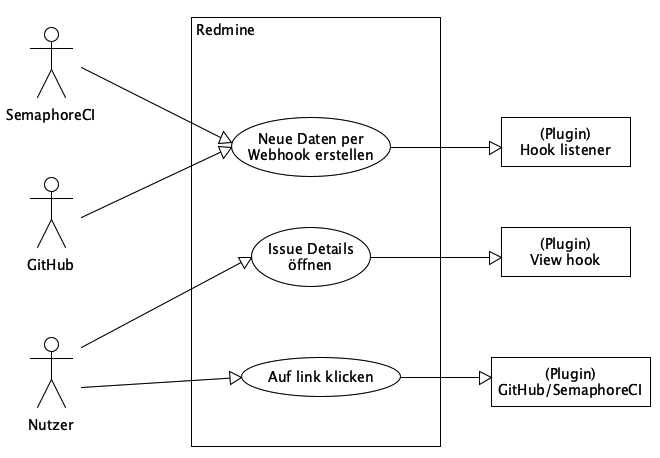
\includegraphics[width=0.8\textwidth]{images/use-case/base.png}
  \caption[Ein Use-Case-Diagramm, welches die verschiedenen Systemanforderungen aufzeigt]{Use-Case-Diagramm mit Systemanforderungen}
  \label{fig:use_case}
\end{figure}
\subsection{Entity-Relationship-Diagram}
Das ERD zeigt die Beziehungen zwischen den einzelnen Entitäten. Da diese PA nur ein Plugin ist, welches neben
bereits bestehenden Entitäten seine eigenen erstellt, wird dort abgegrenzt. Nur Entitäten vom Plugin und
deren Beziehungen werden im ERD dargestellt. \newline
Hier werden drei Optionen aufgezeigt und erklärt, die im Kapitel \ref{chap:decide} (Entscheiden) ausgewertet werden. \newline
Die Attribute wurden auf Basis der Semaphore Webhooks Dokumentation \cite{semaphore_webhooks} und der GitHub Webhooks
Dokumentation über Pull Requests \cite{github_webhooks_pr} erstellt.

\subsubsection{Option 1: Mehrere Entitäten}
Die erste Option ist, dass für Deployments und Pull-Requests eigene Entitäten erstellt werden. Das würde wie folgt aussehen:
\begin{figure}[H]
  \centering
  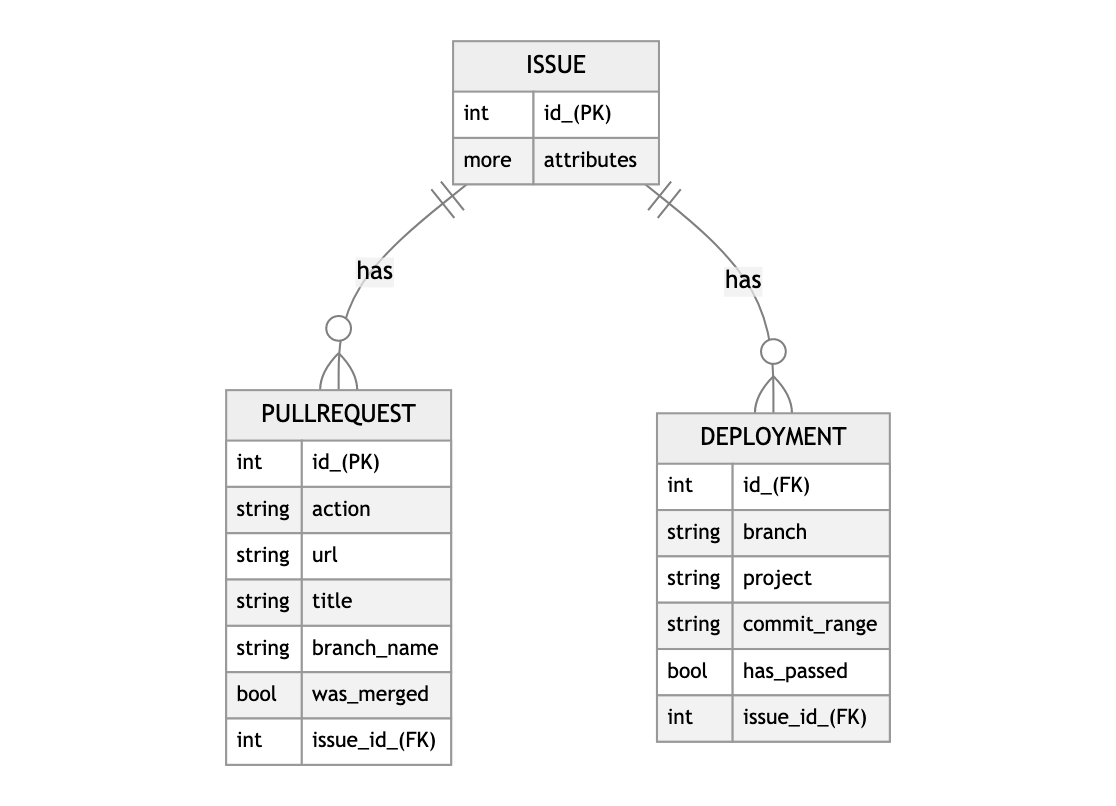
\includegraphics[width=0.8\textwidth]{images/erd/multiple.png}
  \caption[Ein ERD, welches eine separate Entität für Deployments und Pull-Requests aufzeigt.]{ERD mit separaten Entitäten.}
  \label{fig:erd_multiple}
\end{figure}

\subsubsection{Option 2: Inheritance}
Die zweite Option ist, dass für Deployments und Pull-Requests keine eigenen Entitäten erstellt werden, sondern diese von
einer gemeinsamen Entität erben. Das würde wie folgt aussehen:
\begin{figure}[H]
  \centering
  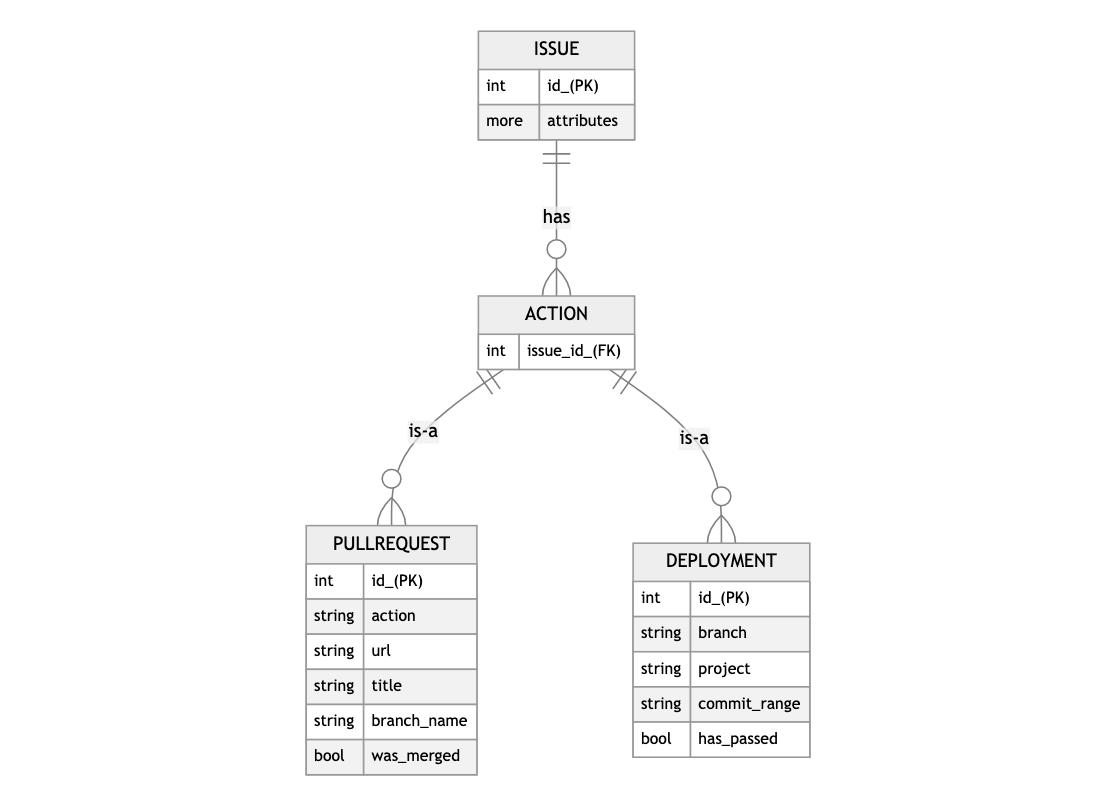
\includegraphics[width=0.8\textwidth]{images/erd/inheritance.png}
  \caption[Ein ERD, welches die Vererbung zwischen Issues und Deployments mit dem Parent Action aufzeigt.]{ERD mit der Vererbung.}
  \label{fig:erd_inheritance}
\end{figure}

\subsubsection{Option 3: Has many through}
Die dritte Option ist, dass Deployments mit einer \enquote{has-many} Beziehung mit Pull-Requests verbunden werden. In diesem Fall hätte jedes
Issue mehrere Deployments \enquote{durch} die Pull-Requests. Daher der Name. Das würde wie folgt aussehen:
\begin{figure}[H]
  \centering
  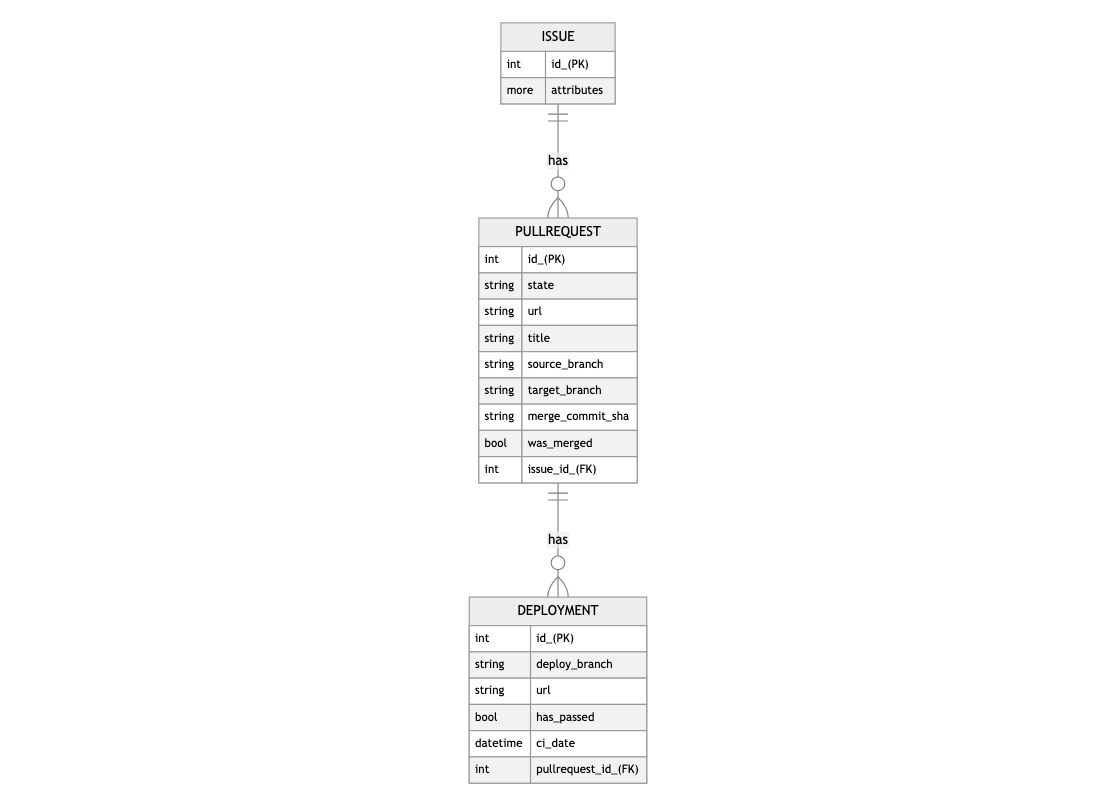
\includegraphics[width=0.8\textwidth]{images/erd/has_many_through.png}
  \caption[Ein ERD, welches die \enquote{has-many-through} Beziehung zwischen Issues und Deployments aufzeigt.]{ERD mit der \enquote{has-many-through} Beziehung zwischen Issues und Deployments.}
  \label{fig:erd_has_many_through}
\end{figure}

\subsection{Activity-Diagram}
\label{sec:activity_diagram}
Das Activity-Diagramm zeigt den Ablauf des Plugins. In diesem Fall gibt es zwei Abläufe:
\begin{itemize}
  \item Hook von SemaphoreCI oder GitHub
  \item Abfragen der Issues
\end{itemize}

\subsubsection{Hook call}
Die Hook Calls werden von SemaphoreCI oder GitHub ausgelöst. Beide bei unterschiedlichen Events, welche beide mit Sanduhren
dargestellt wurden:
\begin{figure}[H]
  \centering
  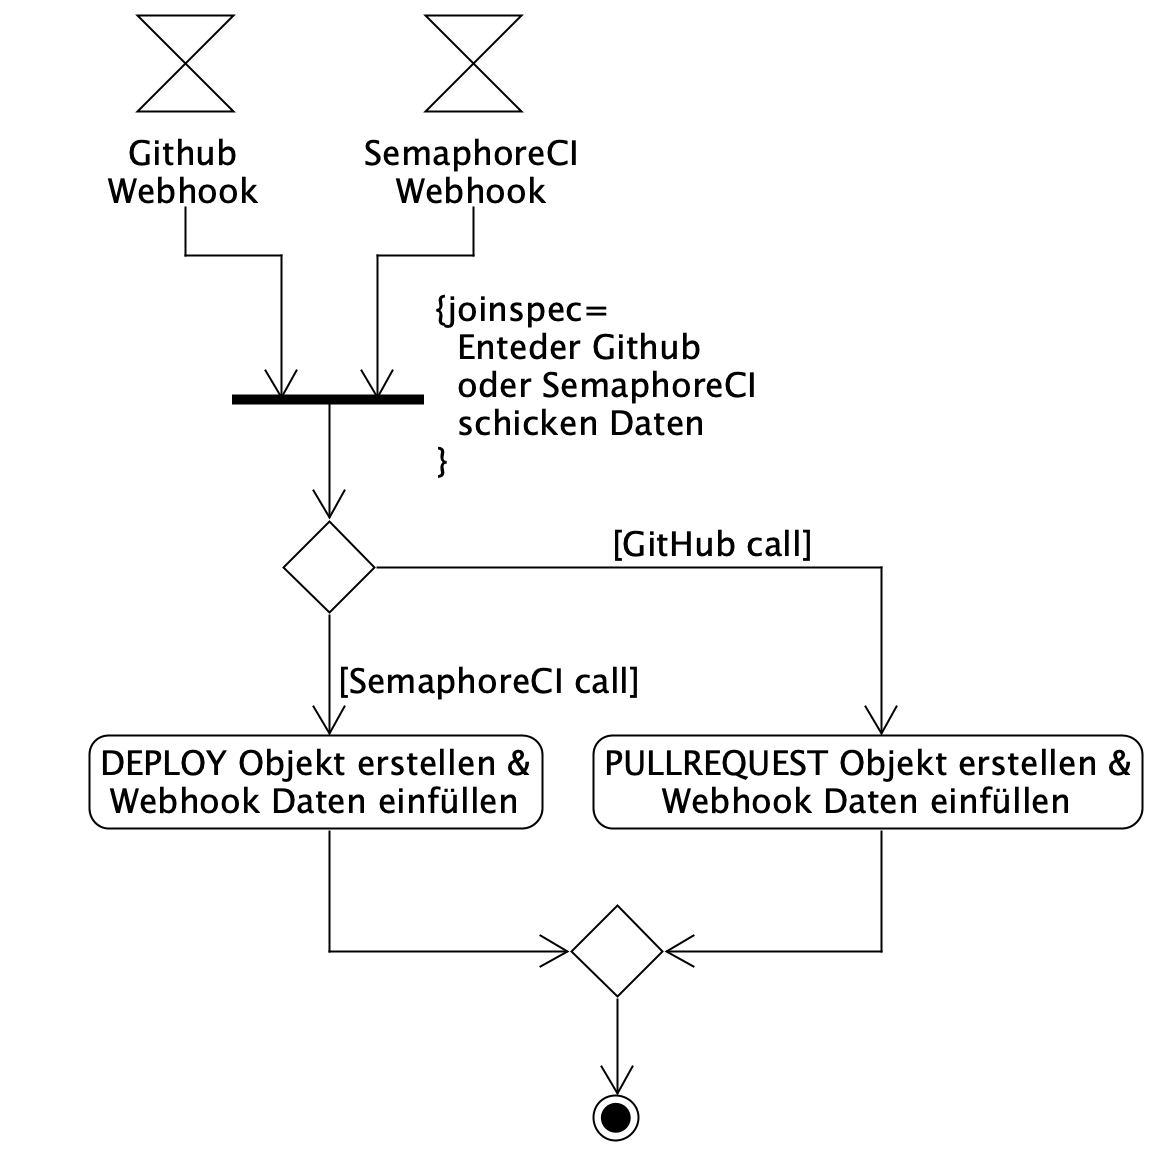
\includegraphics[width=0.8\textwidth]{images/activity/webhook.png}
  \caption[Ein Activity-Diagramm, auf welchem die Verarbeitung der Webhook Daten aufgezeigt wird.]{Activity-Diagramm, welches das Speichern der Daten aufzeigt.}
  \label{fig:activity_hook_call}
\end{figure}

\subsubsection{SemaphoreCI Plan B}
Da SemaphoreCI in den Webhook Daten nicht alle Commit-Hashes, sondern nur eine Range mitliefert, kann es sein, dass die
Informationen, über welche Commits Deployed wurden, nicht vorhanden sind. Deswegen wird hier ein zweiter Vorschlag für den
SemaphoreCI Workflow präsentiert. Dieser würde direkt auf GitHub nachfragen, wie die Commit-History aussieht. So
ungefähr würde das aussehen:
\begin{figure}[H]
  \centering
  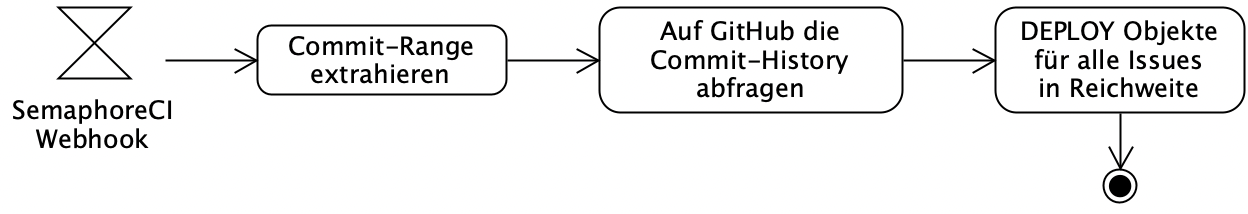
\includegraphics[width=0.8\textwidth]{images/activity/semaphore-backup-hooks.png}
  \caption[Ein Activity-Diagramm, welches den Backup-Plan für SemaphoreCI aufzeigt.]{Activity-Diagramm für den Backup-Plan von SemaphoreCI.}
  \label{fig:activity_plan_b}
\end{figure}
Falls diese Option implementiert wird, ändert sich das Deployment Diagramm ganz leicht, da jetzt
eine neue Brücke vom Plugin zu GitHub existiert. In Rot markiert ist die neue Brücke:
\begin{figure}[H]
  \centering
  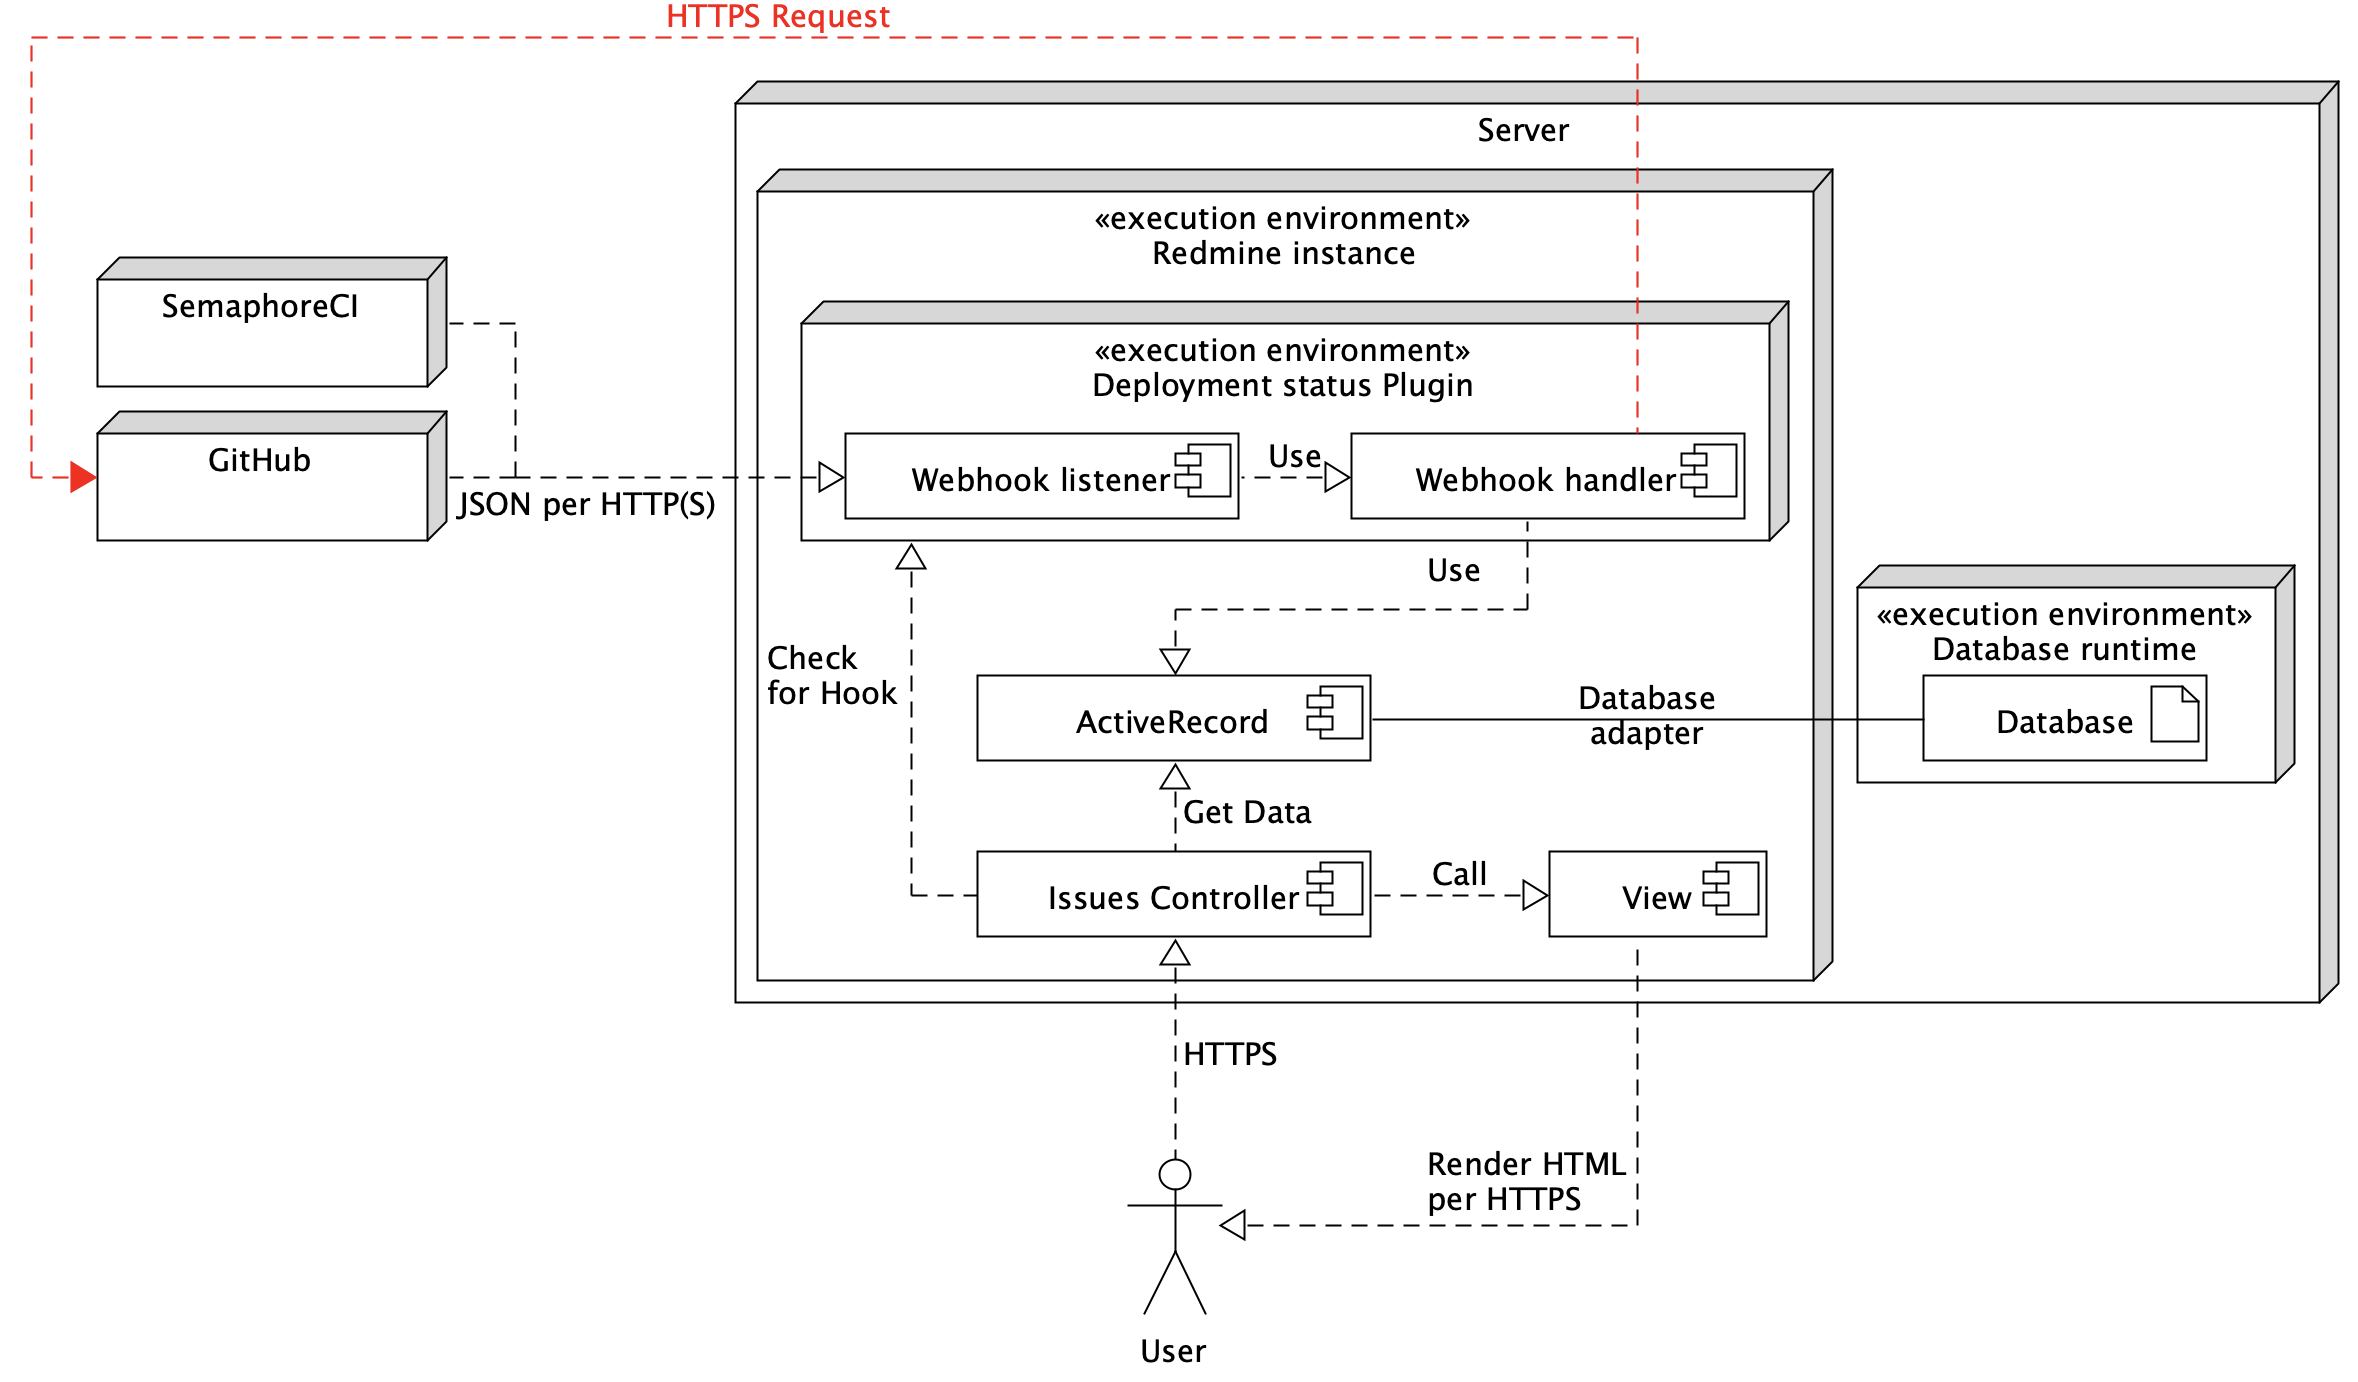
\includegraphics[width=0.8\textwidth]{images/deployment/backup-hooks.png}
  \caption[Das Deployment Diagramm aus \ref{fig:deployment-diagram} mit der neuen Brücke in Rot gekennzeichnet.]{Deployment Diagramm mit der neuen Brücke.}
  \label{fig:activity_plan_b_deployment}
\end{figure}

\newpage
\subsubsection{Abfrage der Issues}
Falls der Nutzer auf die Details eines Issues klickt, wird eine Abfrage an das Plugin gesendet, welches die Pull Requests sowie
Deployments abfragt und diese zurückgibt:
\begin{figure}[H]
  \centering
  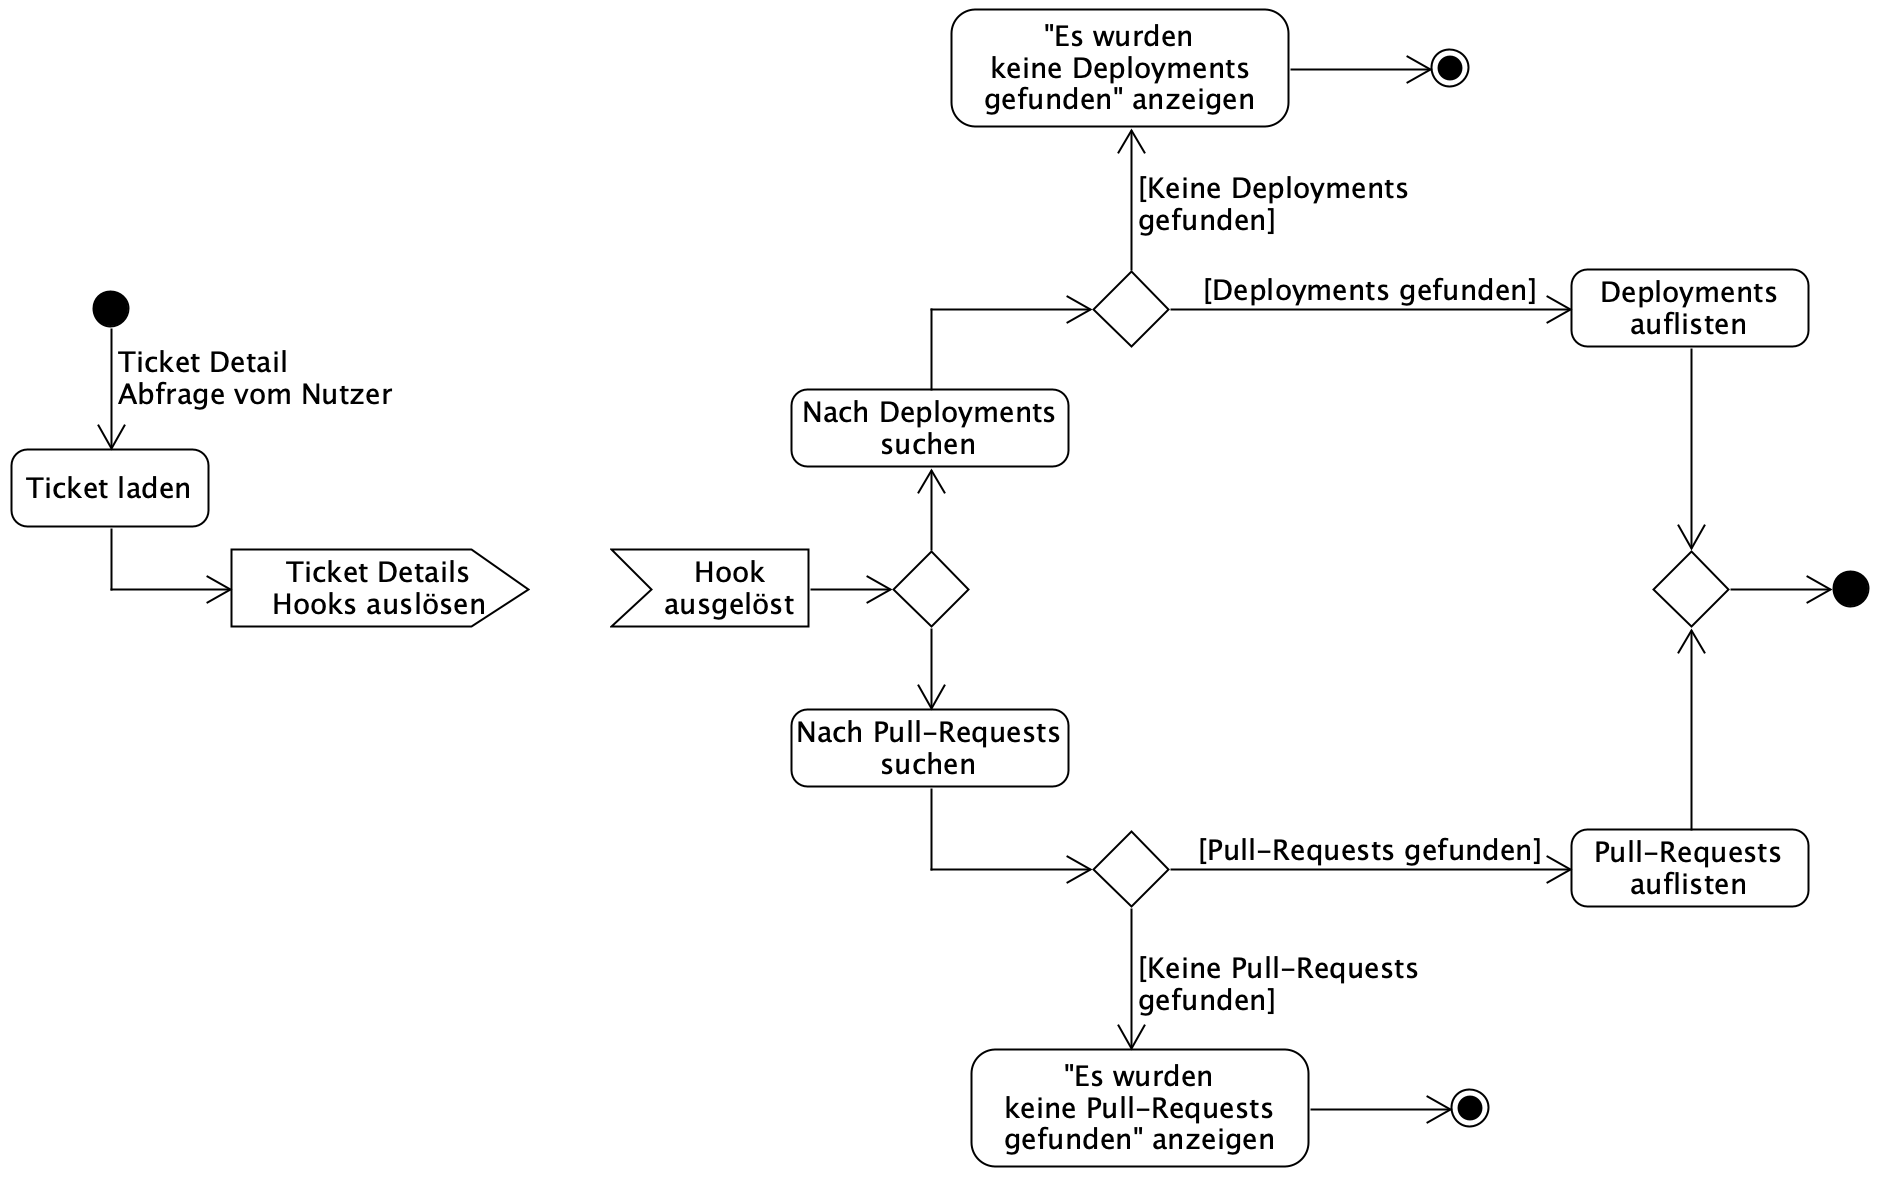
\includegraphics[width=0.8\textwidth]{images/activity/issues-view.png}
  \caption[Activity-Diagramm, welches die Abfrage der Issues darstellt.]{Activity-Diagramm, welches die Abfrage der Issues darstellt.}
  \label{fig:activity_issues}
\end{figure}

\subsection{Mockups}
\label{sec:mockups}
Damit das UI besser geplant werden kann, wird dieses mit Mockups visualisiert. Diese Mockups sollen
nur ungefähr wiedergeben, wie das UI aussehen soll. Da das Plugin auf einer bereits existierenden 
Ansicht aufbaut, nämlich der Issue-View, wird diese nur sehr abstrahiert dargestellt. \newline
Die bereits existierende Ansicht ist in der Abbildung mit weniger Opazität dargestellt.

\newpage
\subsubsection{Option 1: Zwei Listen}
Option eins ist, dass die Pull-Requests und Deployments in zwei Listen dargestellt werden. Das würde ungefähr so
aussehen:
\begin{figure}[H]
  \centering
  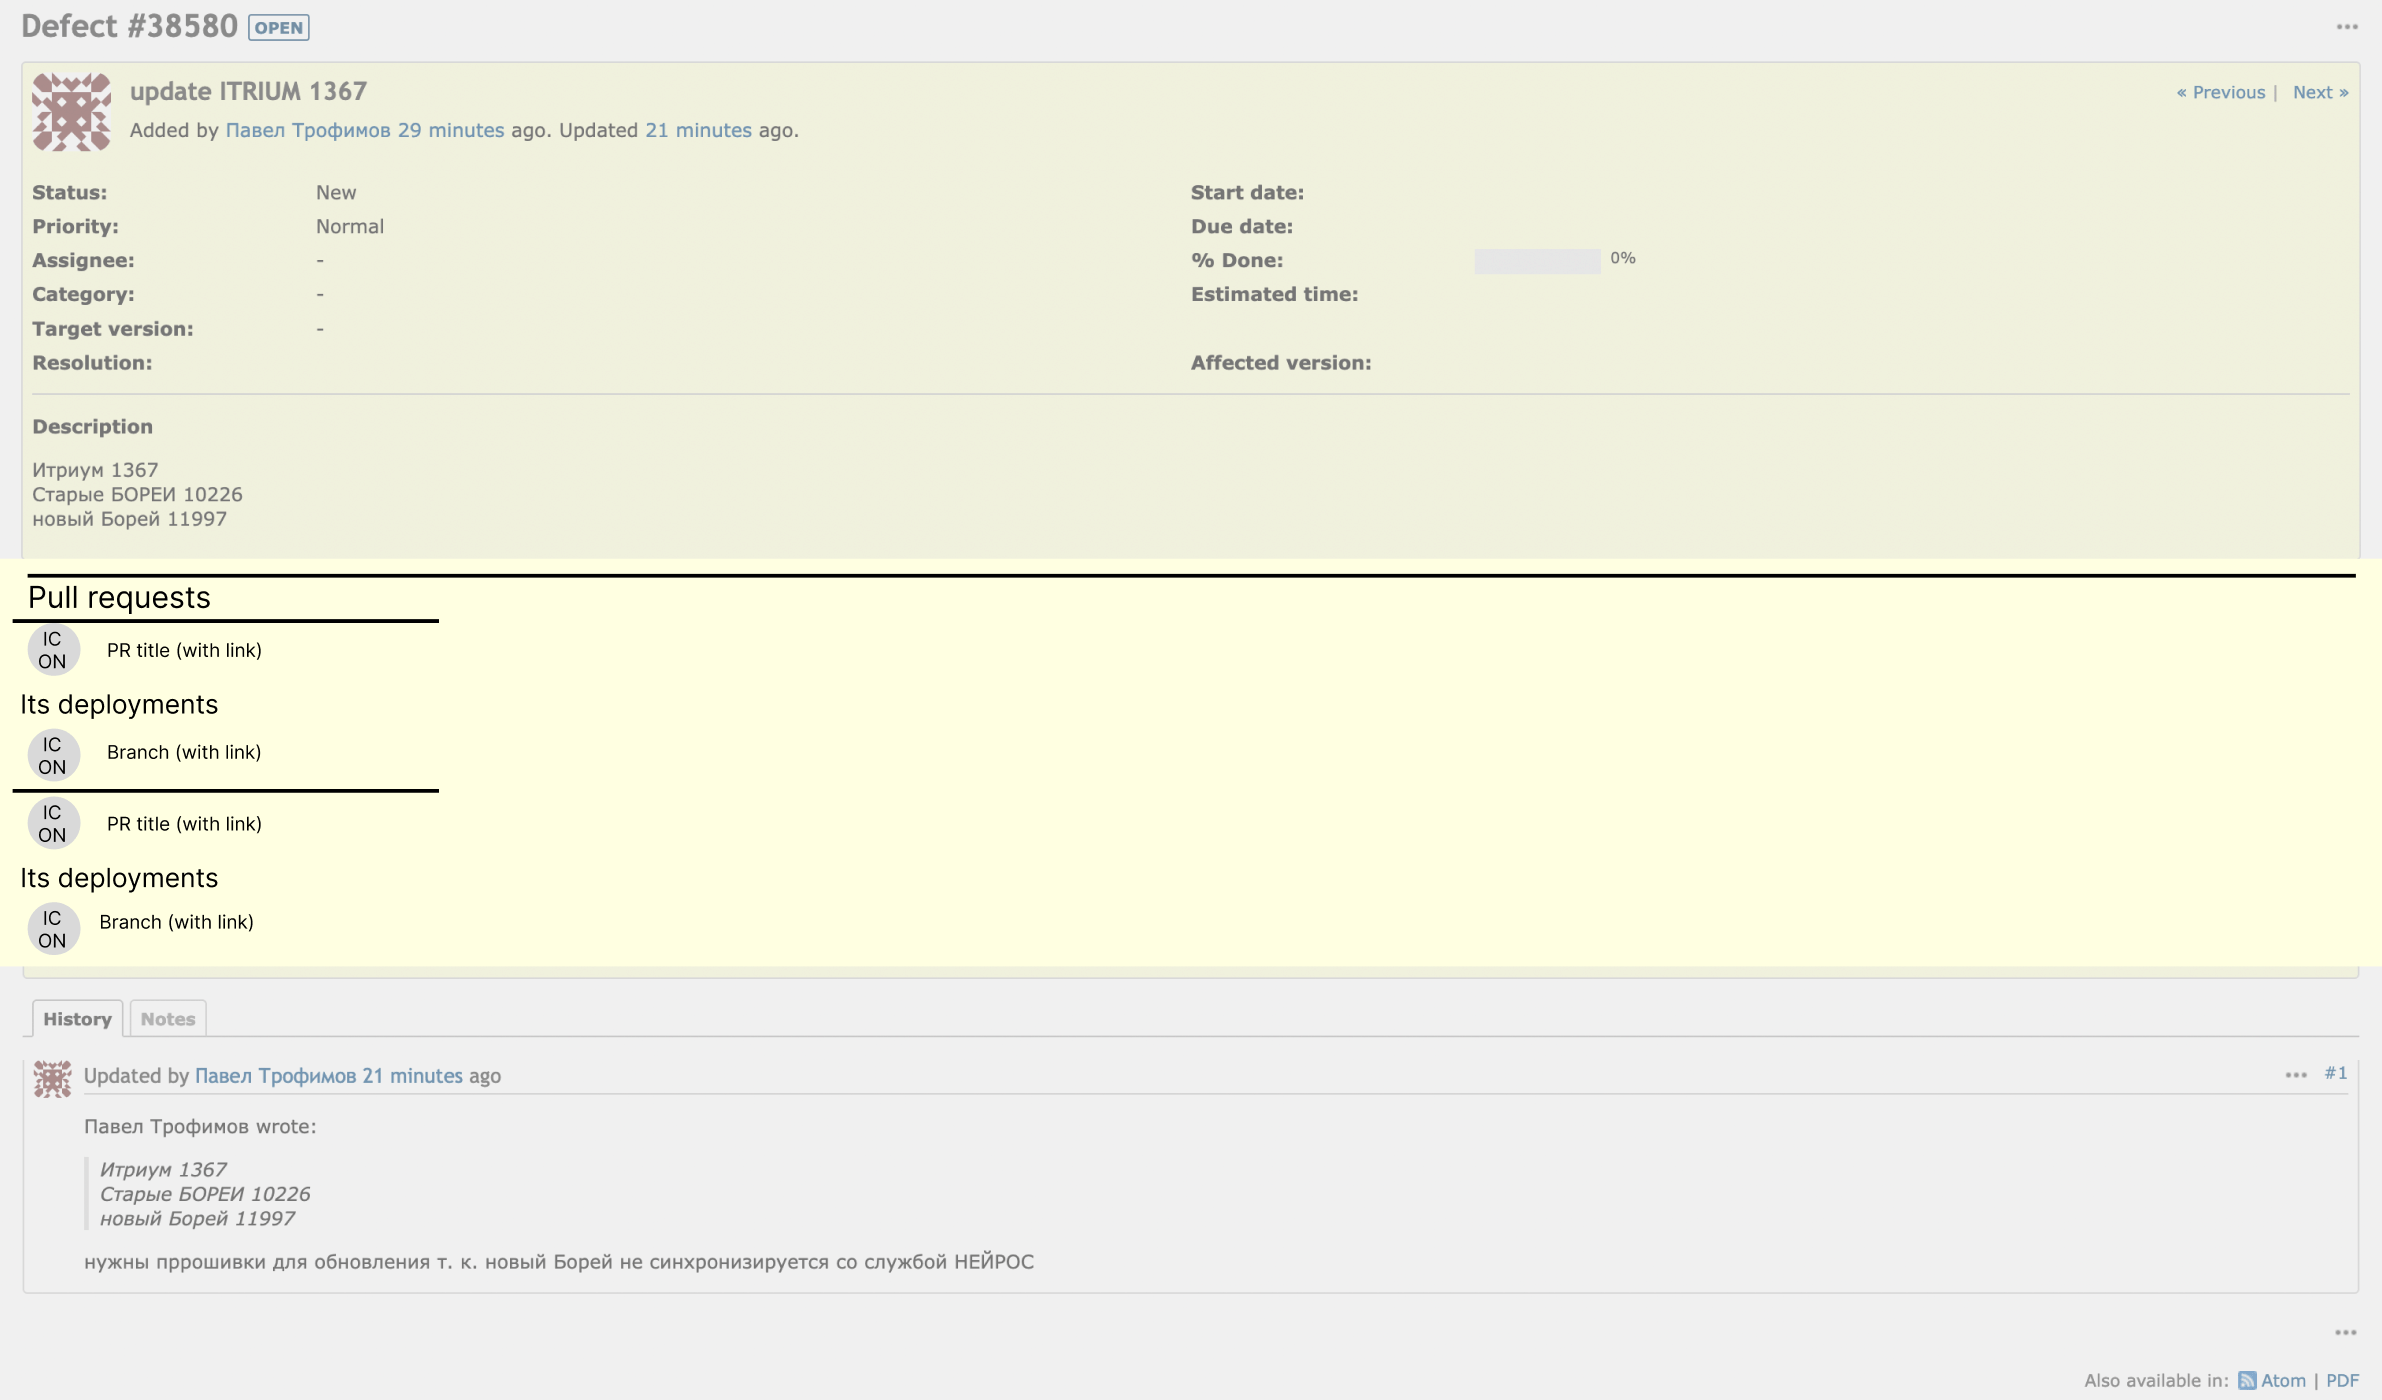
\includegraphics[width=0.8\textwidth]{images/mockup/multiple-lists.png}
  \caption[Ein Mockup, bei welchem die Deployments und Pull Requests separate Listen haben.]{Mockup vom Zwei-Listen-Design.}
  \label{fig:mockup_multi_lists}
\end{figure}

\subsubsection{Option 2: Eine Liste mit Unterlisten}
Die zweite Option ist, dass die Pull Requests aufgelistet werden und die Deployments als Unterlisten aufgelistet
werden. So würde das aussehen:
\begin{figure}[H]
  \centering 
  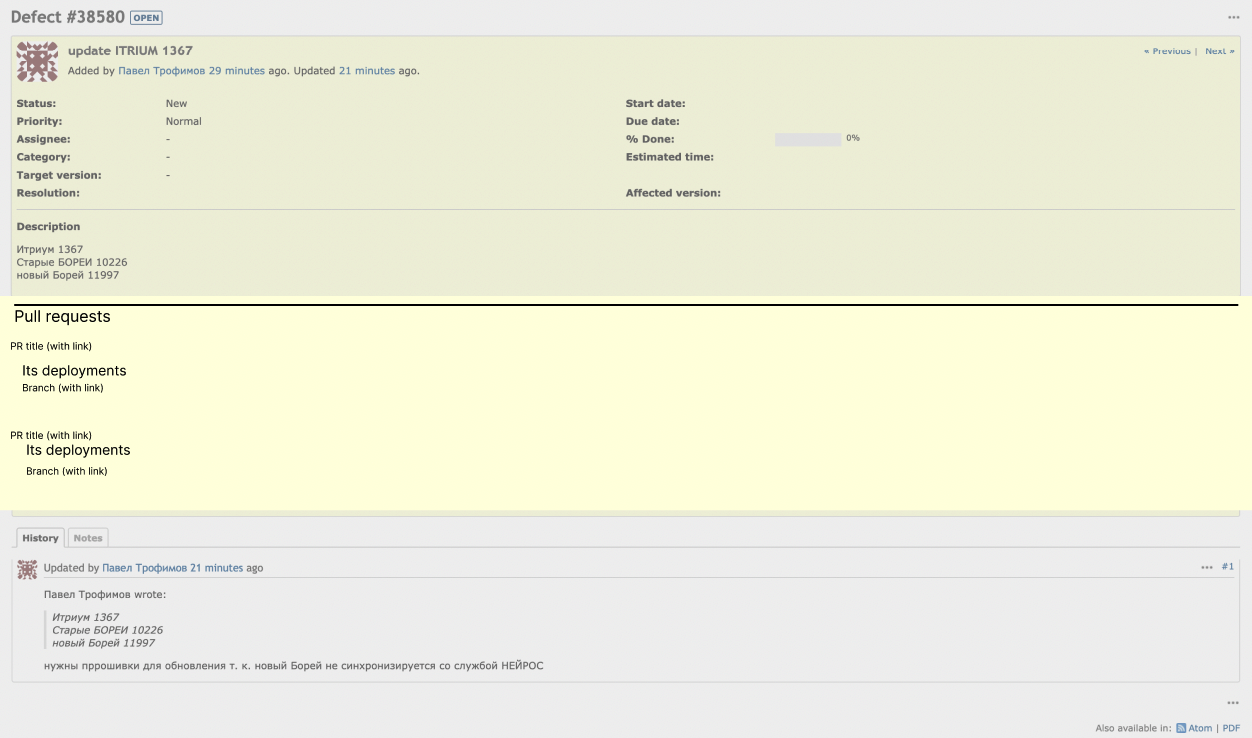
\includegraphics[width=0.8\textwidth]{images/mockup/sublists.png}
  \caption[Ein Mockup, bei welchem die Deployments als Unterlisten aufgelistet werden.]{Mockup vom Sublisten-Design.}
  \label{fig:mockup_sublists}
\end{figure}

\section{Testkonzept}
\label{sec:testkonzept}
Das Testkonzept beschreibt, wie und mit welchen Werkzeugen das Resultat auf seine Richtigkeit kontrolliert wird.

\subsection{Testmittel}
Als Testmittel werden folgende Tools verwendet:
\begin{itemize}
  \item \textbf{Redmine} für das Erstellen von Issues
  \item \textbf{GitHub} für das Erstellen von Repositories und Pull Requests
  \item \textbf{SemaphoreCI} für das Erstellen von Pipelines
  \item \textbf{ngrok} für das Erstellen von HTTP-Tunnels
\end{itemize}

\subsection{Testumgebung}
Die Testumgebung unterscheidet sich zwischen den automatisierten und manuellen Tests.
\subsubsection{Automatisierte Tests}
Die automatisierten Tests werden auf SemaphoreCI ausgeführt. Diese laufen auf einem Ubuntu Server, welcher eine
\enquote{semaphore.yml} Datei hat. Diese Datei definiert, welche Schritte ausgeführt werden sollen.
\subsubsection{Manuelle Tests}
Die manuellen Tests werden auf dem lokalen Gerät des Kandidaten ausgeführt. Dieses Gerät läuft auf MacOS und nutzt
den Firefox, sowie Chrome Browser um die Kompatibilität zu testen.

\subsection{Automatisierte Tests}
Es werden automatisierte Tests für das Plugin geschrieben, welche die Funktionalität der Applikation testen.
Diese werden mit den gleichen Frameworks wie die vom Redmine geschrieben. Das heisst, dass die Tests mit
folgenden Frameworks geschrieben werden:
\begin{itemize}
  \item \textbf{MiniTest} für die Unit-Tests
  \item \textbf{Capybara} für die System-Tests
\end{itemize}
Die Coverage sollte 100\% betragen (bei Klassen über 5 Zeilen). Diese Tests werden dann automatisch auf 
SemaphoreCI ausgeführt. Von der CI erhalten wir dann einen Coverage-Report, sowie eine Liste der
fehlgeschlagenen Tests. Nur falls alles in Ordnung ist, kann man die Pull-Request mergen.

\subsubsection{Weitere Tools}
Tools, welche nicht von Redmine selbst verwendet werden, welche aber dennoch im Plugin verwendet werden, sind:
\begin{itemize}
  \item \textbf{Faker} für das Erstellen von realistischen Testdaten.
  \item \textbf{FactoryBot} für das Initialisieren von Objekten.
\end{itemize}
Die Coverage, sowie andere wichtige Informationen werden unter \ref{sec:automated-tests} dokumentiert.

\subsection{Manuelle Tests}
\label{sec:manual-testing}
Während der Entwicklung und für allfällige Demonstrationszwecke werden manuelle Tests durchgeführt. Diese
werden in diesem Kapitel beschrieben und unter \ref{sec:manual-tests} protokolliert.

\subsubsection{Allgemeiner Vorgang (Vorraussetzungen)}
\label{sec:general-testing}
Um die Funktionalität des Plugins zu testen, muss eine eintreffende Webhook von SemaphoreCI oder GitHub simuliert werden.
Dabei hat man zwei Optionen:
\begin{itemize}
  \item \st{Senden von Daten per HTTP-Request an den lokalen Server}
  \item Benützen des Dienstes, damit dieser die Daten schickt
\end{itemize}

\textbf{Senden von Daten per HTTP-Request an den lokalen Server} \\
Option eins ist das manuelle Senden von Daten an den lokalen Server. Dies kann man in der Konsole mit dem curl Programm
\cite{everything_curl} machen. Dies ist jedoch eine sehr aufwändige und ungenaue Art zu testen, weshalb diese Option nicht
weiter verfolgt wird. \newline

\textbf{Benützen des Dienstes, damit dieser die Daten schickt} \\
Die zweite Option ist, ein Repository auf GitHub zu erstellen und dieses mit SemaphoreCI / Github Webhooks zu
verbinden. \newline
Damit dann diese Daten beim lokalen Server ankommen können, müsste man mit ngrok \cite{ngrok_http_docs} einen HTTP-Tunnel
erstellen, welcher eine öffentliche IP zur Verfügung stellt. \newline
Diese Methode ist auch sehr aufwändig, doch liefert genauere Daten als Option eins, weshalb diese benutzt wird.

\subsubsection{1. Verarbeiten von SemaphoreCI Daten}
Da unter Kapitel \ref{sec:general-testing} etabliert wurde, dass die Dienste wirklich verwendet werden beim manuellen Testen,
wird der Test nach folgenden Schritten durchgeführt:
\begin{enumerate}
  \item Ein Issue auf Redmine erstellen
  \item Auf GitHub ein Repository erstellen und dieses mit SemaphoreCI verbinden. 
  (\textbf{Wichtig:} Es muss ein Deploy-Skript erstellt werden. Dieses heisst wie folgt:
  [branchname]-deploy.yml)
  \item Eine Pull Request erstellen und mergen.
  \item Warten, bis die Pipeline auf SemaphoreCI durchgelaufen ist
  \item Auf dem Issue kontrollieren, ob die Daten korrekt angezeigt werden
\end{enumerate}

\textbf{Das zu erwartende Resultat ist,} dass in der Beschreibung des Issues ein Deployment sichtbar wird. Das kann entweder grün oder rot
sein, je nachdem, ob die Pipeline erfolgreich durchgelaufen ist oder nicht.

\subsubsection{2. Verarbeiten von GitHub Daten}
\label{sec:github-testing}
Das Testen von den GitHub Webhooks lauft sehr ähnlich ab:
\begin{enumerate}
  \item Ein Issue auf Redmine erstellen
  \item Auf GitHub ein Repository erstellen
  \item Eine GitHub Webhook erstellen, welche bei Pull Requests Daten schickt. (Die URL muss auf den lokalen Server zeigen)
  \item Einen feature Branch erstellen (\textbf{Wichtig:} Die Issue-Nummer muss im Branchnamen enthalten sein)
  \item Eine Pull Request erstellen
  \item Auf dem Issue kontrollieren, ob die Daten korrekt aufgelistet werden
\end{enumerate}

\textbf{Das zu erwartende Resultat ist,} dass in der Beschreibung des Issues eine Pull Request angezeigt wird. Da diese noch nicht gemerged
wurde, sollte es sichtbar sein, dass die Pull Request offen ist.

\subsubsection{3. Der Nutzer schaut sich ein Issue an mit Daten}
Für diesen Testfall wird auf einer lokalen Redmine Instanz ein Issue erstellt. Daraufhin werden die Schritte aus
\ref{sec:github-testing} durchgeführt, damit das Issue mit Daten vom Plugin befüllt wird. \newline
\textbf{Das zu erwartende Resultat ist,} dass die offene Pull Request angezeigt wird. Das sollte ohne grosse Ladezeit passieren, wie von 
Software-Design Anforderung drei verlangt.

\subsubsection{4. Der Nutzer schaut sich ein Issue an ohne Daten}
Für diesen Testfall wird auf einer lokalen Redmine Instanz ein Issue erstellt. Dann wird in der Beschreibung des Tickets
kontrolliert, was angezeigt wird. \newline
\textbf{Das zu erwartende Resultat ist,} dass keine Daten angezeigt werden.

\subsubsection{5. Das Plugin funktioniert mit Redmine Version 4, sowie 5}
Für diesen Testfall wird die lokale Redmine Instanz auf Version 4 gesetzt. Dann wird das Plugin getestet. Es wird
alles was in Fällen 1-4 getestet wurde, nochmals getestet. \newline
\textbf{Das zu erwartende Resultat ist,} dass alles funktioniert wie in den Fällen 1-4.

\subsubsection{6. Das Plugin funktioniert auf Chrome, sowie Firefox}
Für diesen Testfall werden Tests 3 und 4 auf Chrome und Firefox durchgeführt. Es müssen nur Fälle 3 und 4
ausgeführt werden, da die anderen nur im Backend etwas machen und dieser Testfall das UI testet. \newline
\textbf{Das zu erwartende Resultat ist,} dass alles funktioniert wie in den Fällen 3 und 4.

\subsection{Was bewusst nicht getestet wird}
Da Git ein sehr komplexes System ist, werden bestimmte Edge-Cases nicht getestet. Damit ist hauptsächlich
die Änderung von Git-History gemeint. Da das ohnehin nicht getan werden sollte, sprengt das den Rahmen
dieser Arbeit. Das wäre aber eine gute Erweiterung für das Plugin.

  \chapter{Entscheiden}
\label{chap:decide}
In diesem Kapitel werden Entscheidungen und dessen Begründungen dokumentiert. \newline
Da diese PA ein Plugin für bereits etablierte Software ist, gibt es, vor allem bezüglich des Tech-Stacks, nicht viel zu
entscheiden. Wie die zweite Software-Design Anforderung besagt: \enquote{Das Plugin soll sich an die Coding-Guidelines von
Redmine halten...} \newline
Für das Bewerten wurden alle Optionen vorgelegt und kurz beschrieben. Dann wurde mit einer Entscheidungsmatrix
bewertet und gewählt.

\section{Bewertungen}
\subsection{Entity-Relationship-Diagram}
\subsubsection{Option 1: Mehrere Entitäten}
Die erste Option, wie auf Grafik \ref{fig:erd_multiple} zu sehen, ist, dass für Deployments und Pull-Requests
eigene Entitäten erstellt werden, welche beide direkt mit den Issues verbunden sind. \newline
Die Vorteile dieser Option sind beispielsweise, dass die Komplexität der Datenstruktur gering ist. Es ist einfach zu
implementieren und eventuellen späteren Entwicklern zu erklären. \newline
Ein grosser Nachteil dieser Datenstruktur ist, dass wahrscheinlich zwei separate Kontroller erstellt werden müssen, was
die Codebase unnötig vergrössert (aber nicht unbedingt Komplexität hinzufügt).

\subsubsection{Option 2: Inheritance}
Die zweite Option, wie auf Grafik \ref{fig:erd_inheritance} zu sehen, ist, dass für Deployments und Pull-Requests nur
Child-Entitäten erstellt werden, welche beide von einer gemeinsamen Entität erben. \newline
Der grösste Vorteil dieser Option ist, dass die Vererbung die Codebase vereinfachen kann, falls richtig implementiert.
\newline
Nachteile sind, dass die Komplexität der Datenstruktur massiv erhöht wird. Vererbung ist in Datenbanken nicht üblich, was
implementationen davon erschwert. Rails würde dabei einen grossen Teil er Arbeit abnehmen, dennoch bleibt die Komplexität
hoch.

\subsubsection{Option 3: Has many through}
\label{sec:decide_has_many_through}
Die dritte und letzte Option, dargestellt auf Grafik \ref{fig:erd_has_many_through}, ist die am meisten an Rails angelehnte
Methode. Dabei wäre ein Deployment nicht mehr mit dem Issue, sondern der Pull Request verbunden. Die Verbindung zwischen
einem Issue und einem Deployment würde somit \enquote{durch} die Pull Request gehen. Deswegen das \enquote{through} im Namen.
Diese Option ist möglich, da wir Pull Requests deployen und nicht Issues. \newline
Vorteilhaftig wäre, dass die Datenstruktur besser die Realität abbildet. In der Realität wird eine Pull Request Deployed,
was in der Datenstruktur auch so dargestellt wäre. \newline
Ein grosses Problem an diesem Ansatz ist, dass diese Option sehr viel von der Datenbank lesen muss. Bei grossen Systemen
kann das eventuell zu Performance-Problemen führen.

\subsection{Activity-Diagram}
Die Acticity-Diagramme unter Kapitel \ref{sec:activity_diagram} zeigen mehr oder weniger die einzige Möglichkeit auf den
Prozess zu gestalten. Im Design dieses Projektes muss man sich viel externen Prozessen anpassen; Redmine gibt den
Issue-Prozess vor und GitHub sowie SemaphoreCI die Webhook Prozesse.

\subsection{Tech-Stack}
Der Tech-Stack wird bereits von Redmine vorgegeben. Es wird Ruby on Rails mit ERB als Template-Engine verwendet. Ausserdem
wird MiniTest mit Capybara für die Tests verwendet. \newline
Die einzige Freiheit, welche geboten wird ist die Wahl der Datenbank.

\subsection{UI}
Obwohl der Grossteil der UI bereits von Redmine vorgegeben wird, wird ein Teil selbst gestaltet. Die Mockups unter Kapitel
\ref{sec:mockups} zeigen zwei Möglichkeiten bezüglich der UI auf. \newline
Es gibt hier nicht viel zu entscheiden, da es eine Sache von persönlicher Präferenz ist. Dennoch haben beide Optionen
Vor- und Nachteile. \newline

\subsubsection{Option 1: Zwei Listen}
Die erste Option, illustriert auf Grafik \ref{fig:mockup_multi_lists}, zeigt zwei Listen. Eine für die Pull Requests und
die zweite darunter für Deployments. \newline
Während es besser voneinander getrennt ist, wird es schwierig zu wissen, zu welcher Pull Request welcher Deployment
gehört. \newline

\subsubsection{Eine Liste mit Unterlisten}
Die zweite Option wird auf Grafik \ref{fig:mockup_sublists} dargestellt. Bei dieser gibt es nur eine Liste, welche
die Pull Requests auflistet. Jede Pull Request hat eine Liste von vergangenen Deployments und dessen Status. \newline
Obwohl diese Option schnell sehr unübersichtlich aussehen kann, hat man den Vorteil das die Deployments jeder
Pull Request einfacher zuzuordnen sind. \newline

\section{Entscheidungen}
\subsection{Entity-Relationship-Diagram}
\label{sec:decide_erd}
\subsubsection{Bewertungsmatrix}
\begin{center}
    \resizebox{0.75\textwidth}{!}{%
        \begin{tabular}{|c|c|c|c|c|}
            \hline
            \textbf{Kriterium} & \textbf{Gewichtung} & \textbf{Option 1} & \textbf{Option 2} & \textbf{Option 3} \\ \hline
            Einfachheit & 30\% & 7.5 & 5 & 7 \\ \hline
            Realitätsnähe & 35\% & 5 & 7.5 & 10 \\ \hline
            Erweiterbarkeit & 35\% & 7.5 & 5 & 8 \\ \hline
            \textbf{Total} & --- & 6.625 & 5.875 & \textbf{8.4} \\ \hline
        \end{tabular}%
    }
\end{center}
\subsubsection{Entscheidung}
Die Entscheidung fiel auf die dritte Option (Kapitel \ref{sec:decide_has_many_through}), da diese die Realität am besten
abbildet, es einfacher zu erweitern ist und die Implementation ausserdem nicht sehr komplex ist. \newline
Langfristig wird die Codebase dadurch profitieren, da die Datenstruktur einfacher zu verstehen ist und die Komplexität
tiefer ist. \newline

\subsection{Activity Diagramme}
Zu den Activity Diagrammen gibt es nichts zu entscheiden, ausser wie SemaphoreCI implementiert wird,
da wahrscheinlich ein Backup-Plan nötig ist. \newline
Momentan fehlen Informationen darüber, ob die Implementation möglich ist, weshalb die GitHub Implementation als erstes
stattfinden wird. Danach wird während der Implementation von SemaphoreCI entschieden, ob es möglich ist oder nicht. Falls
nicht, wird der Backup-Plan implementiert. \newline

\subsection{Tech-Stack}
Die Entscheidung für den Tech-Stack ist bereits gefallen, da Redmine diesen vorgibt. \newline
Die Datenbank für die CI, sowie das lokale testen wird PostgreSQL sein, da dass der Standard bei der Renuo AG ist.
\newline

\subsection{Mockups}
\subsubsection{Bewertungsmatrix}
\begin{center}
    \resizebox{0.75\textwidth}{!}{%
        \begin{tabular}{|c|c|c|c|}
            \hline
            \textbf{Kriterium} & \textbf{Gewichtung} & \textbf{Zwei Listen} & \textbf{Unterlisten} \\ \hline
            Übersichtlichkeit & 40\% & 8 & 7 \\ \hline
            Zuordnung & 50\% & 6 & 10 \\ \hline
            Ästhetik & 10\% & 8 & 9 \\ \hline
            \textbf{Total} & --- & 7 & \textbf{8.7} \\ \hline
        \end{tabular}%
    }
\end{center}

\subsubsection{Entscheidung}
Option zwei, aus Grafik \ref{fig:mockup_sublists}, wurde gewählt, da die Deployments besser zu den Pull Requests
zugeordnet werden können. Der Nachteil ist, dass es sehr schnell sehr unübersichtlich werden kann, doch in der Realität
hat es zu jedem Issue meistens eine Pull Request, weshalb das kein grosses Problem darstellt.

  \chapter{Realisieren}
In diesem Kapitel geht es um die Implementation der Software. Diese wird nach den Diagrammen aus dem Kapitel
\ref{chap:plan}, Planen.

\section{Entwicklungsumgebung}
\subsection{Versionierung}
Für die Versionierung wird Git verwendet. Dabei wird GitHub als Remote-Repository verwendet. Das Repository mit
dem Source-Code kann unter \url{https://github.com/aneshodza/gnosis} gefunden werden.

\subsection{IDE}
Als IDE wird vim mit verschiedenen Plugins verwendet. Bestimmte Sachen wurden in der \bgmintinline{bash}{.vimrc} Datei
konfiguriert, damit die Arbeit möglichst effizient ist. \newline
Diese Konfigurationen sind unter \newline
\url{https://github.com/aneshodza/.dotfiles/blob/ad87ee9ecc5588a59d66e211797792099569ca95/.vimrc} zu finden.

\subsection{CI/CD}
Für die CI/CD Pipeline wird SemaphoreCI verwendet. Das ist passend, da auch die PA sehr eng mit SemaphoreCI verbunden
ist.

\begin{minipage}{\textwidth}
  \section{Aufsetzen des Projektes}
  Zu Beginn wird Arbeitspaket 7, Aufestzen des Projektes, implementiert. Dazu sind folgende Schritte zu befolgen:
  \begin{enumerate}
    \item Erstellen des Plugins
    \item Erstellen des Remote-Repository
    \item Mit dem README beginnen
    \item Aufsetzen der CI/CD Pipeline \newline
  \end{enumerate}
\end{minipage}

\begin{minipage}{\textwidth}
  \subsection{Erstellen des Plugins}
  Um das Plugin aufzusetzen begeben wir uns in das Verzeichnis der Lokalen Redmine Instanz. Diese wurde in den
  Vorarbeiten bereits erstellt und aufgesetzt. \newline
  Dort wird mit dem Befehl \bgmintinline{bash}{bundle exec rake generate redmine_plugin gnosis} das Plugin erstellt. Der
  Konsolen-Output sieht wie folgt aus:
  \begin{codebox}[]
    \begin{minted}{bash}
> bundle exec rails generate redmine_plugin gnosis
create  plugins/gnosis/app
# Lots of things being created...
create  plugins/gnosis/README.rdoc
# Lots of things being created...
create  plugins/gnosis/test/test_helper.rb
    \end{minted}
  \end{codebox}

  Wenn wir dann mit \bgmintinline{bash}{cd plugins/gnosis} in das Plugin wechseln, sehen wir, dass bestimmte Dateien
  bereits wurden. Diese werden bei Gebrauch erklärt und aufgezeigt.
\end{minipage}

\begin{minipage}{\textwidth}
  \subsection{Erstellen \& Konfigurieren des Repository}
  Das Projekt wird auf GitHub mit Git Versionsverwaltet, weshalb als Erstes ein GitHub Remote-Repository (auch einfach
  Repository genannt) erstellt werden muss. Das wird nach GitHub Dokumentation gemacht \cite{github_create_repo}.

  \subsubsection{Erstellen des Lokalen Repostiory}
  Danach muss das lokale Plugin mit dem Repository verbunden werden. Dazu müssen wir mit der Konsole in das Directory
  unseres Plugin wechseln, welches unter \menu{redmine/plugins/gnosis} zu finden ist. \newline
  Dort initialisieren wir das lokale Repository mit \bgmintinline{bash}{git init} und verbinden es mit dem Remote
  Repository indem wir \bgmintinline{bash}{git remote add origin [URL]} ausführen.

  \subsubsection{Initial Commit}
  Nun können wir den ersten Commit machen. Das können wir ganz einfach mit wenigen Befehlen machen:
  \begin{codebox}[]
    \begin{minted}{bash}
> git add -A
> git commit -m "Initial commit"
> git push -u origin main
    \end{minted}
  \end{codebox}

  \subsubsection{Git-flow initialisieren}
  Das Projekt wird nach der Git-flow Methode versioniert. Das bedeutet, dass der main Branch für die Releases
  verwendet wird und der develop Branch für die Entwicklung. \newline
  Dann hat man auch feature, bugfix und hotfix Branches, welche alle selbsterklärend sind. \newline
  Für jedes AP wird ein feature Branch erstellt, welcher dann in den develop Branch gemerged wird. \newline
  Als erstes müssen wir den develop branch mit \bgmintinline{bash}{git checkout -b develop} erstellen und diesen
  mit \bgmintinline{bash}{git push -u origin develop} auf remote pushen. \newline
\end{minipage}

\begin{minipage}{\textwidth}
  \subsection{Erstellen des README}
  Beim Erstellen des Plugins wurde automatisch ein \enquote{README.rdoc} erstellt. Dieses wird bei Ruby Projekten
  oft anstatt eines \enquote{README.md} verwendet. Da diese PA nach Vorgaben von Redmine arbeitet, wird auch das
  README im rdoc Format geschrieben. \newline
  Da noch nicht viel im Projekt steht, wird nur beschrieben was genau das Plugin kann und wie es funktioniert. \newline
\end{minipage}

\subsection{Aufsetzen der CI/CD Pipeline}
Die CI/CD wird auf SemaphoreCI eingerichtet, weshalb wir uns dort anmelden und ein neues Projekt erstellen. Man kann dieses
direkt mit GitHub verbinden und Semaphore die meiste Arbeit machen lassen.

\subsubsection{Erstellen der \enquote{bin files}}
Da die Tests sowie Linter immer wieder ausgeführt werden, ist es sinnvoll diesen Prozess zu automatisieren. Dazu werden 
\enquote{bin files} erstellt. Diese sind kleine Bash-Scripts, welche repeditive Aufgaben automatisieren. In unserem Fall sind
das die Ausführungen von den Tests und Lintern sowie das aufsetzen des Projektes. \newline

\begin{minipage}{\textwidth}
  Für die Tests wird ein \bgmintinline{bash}{bin/test} mit folgendem Inhalt erstellt:
  \begin{codebox}[]
    \begin{minted}{bash}
#!/bin/bash

white='\033[1;37m'
red='\033[0;31m'
green='\033[0;32m'

rake redmine:plugins:test:functionals
# TODO: Add other types of tests when they are implemented

if [[ $? -eq 0 ]]; then
  echo -e "${green}----------------------------------------"
  echo -e "Tests passed"
  echo -e "----------------------------------------${white}"
else
  echo -e "${red}----------------------------------------"
  echo -e "Tests failed"
  echo -e "----------------------------------------${white}"
  exit 1
fi
    \end{minted}
  \end{codebox}
\end{minipage}

\begin{minipage}{\textwidth}
  Dann braucht es ein \bgmintinline{bash}{bin/fastcheck} für linter und so weiter mit folgendem Inhalt:
  \begin{codebox}[]
    \begin{minted}{bash}
#!/bin/bash

white='\033[1;37m'
red='\033[0;31m'
green='\033[0;32m'

function return_code {
  if [ $? -ne 0 ]; then
    echo -e "${red} Error: $1 found errors! ${white}"
    failing_checks+=("$1")
    passing=false
  fi
}

passing=true
failing_checks=()

echo "Executing fastchecks..."

if [[ $* == *--fix* ]]; then
  echo "Fixing..."
  bundle exec rubocop -a --config .rubocop.yml
  return_code "Rubocop"
else 
  echo "Note: You can use --fix to fix the errors automatically"
  bundle exec rubocop --config .rubocop.yml
  return_code "Rubocop"
fi

bundle exec brakeman -q -z --no-summary --no-pager
return_code "Brakeman"

if [ "$passing" = true ]; then
  echo -e "${green}----------------------------------------"
  echo -e "All checks passed"
  echo -e "----------------------------------------${white}"
  exit 0
  else
  echo -e "${red}----------------------------------------"
  echo -e "Some checks failed"
  echo -e "Failed checks: ${failing_checks[@]}"
  echo -e "----------------------------------------${white}"
  exit 1
fi
    \end{minted}
  \end{codebox}
  
\end{minipage}

\begin{minipage}{\textwidth}
  Dann braucht es ein \bgmintinline{bash}{bin/setup} für das aufsetzen des Projektes mit folgendem Inhalt:
  \begin{codebox}[]
    \begin{minted}{bash}
yarn install
bundle exec rake redmine:plugins:migrate
    \end{minted}
  \end{codebox}
\end{minipage}

\subsubsection{Erstellen der \enquote{semaphore.yml} Datei}
Was wir noch machen müssen, ist die \bgmintinline{bash}{semaphore.yml} Datei zu erstellen. Diese muss ungefähr folgenden Ablauf
ausführen:
\begin{enumerate}
  \item Redmine klonen und Aufsetzen
  \item Postgres starten
  \item Datenbank erstellen und migrieren
  \item In das Plugins directory wechseln
  \item Plugin klonen
  \item Tests ausführen
\end{enumerate}

\begin{minipage}{\textwidth}
  Auf einem Activity Diagramm würde das so aussehen: \newline
  \begin{center}
    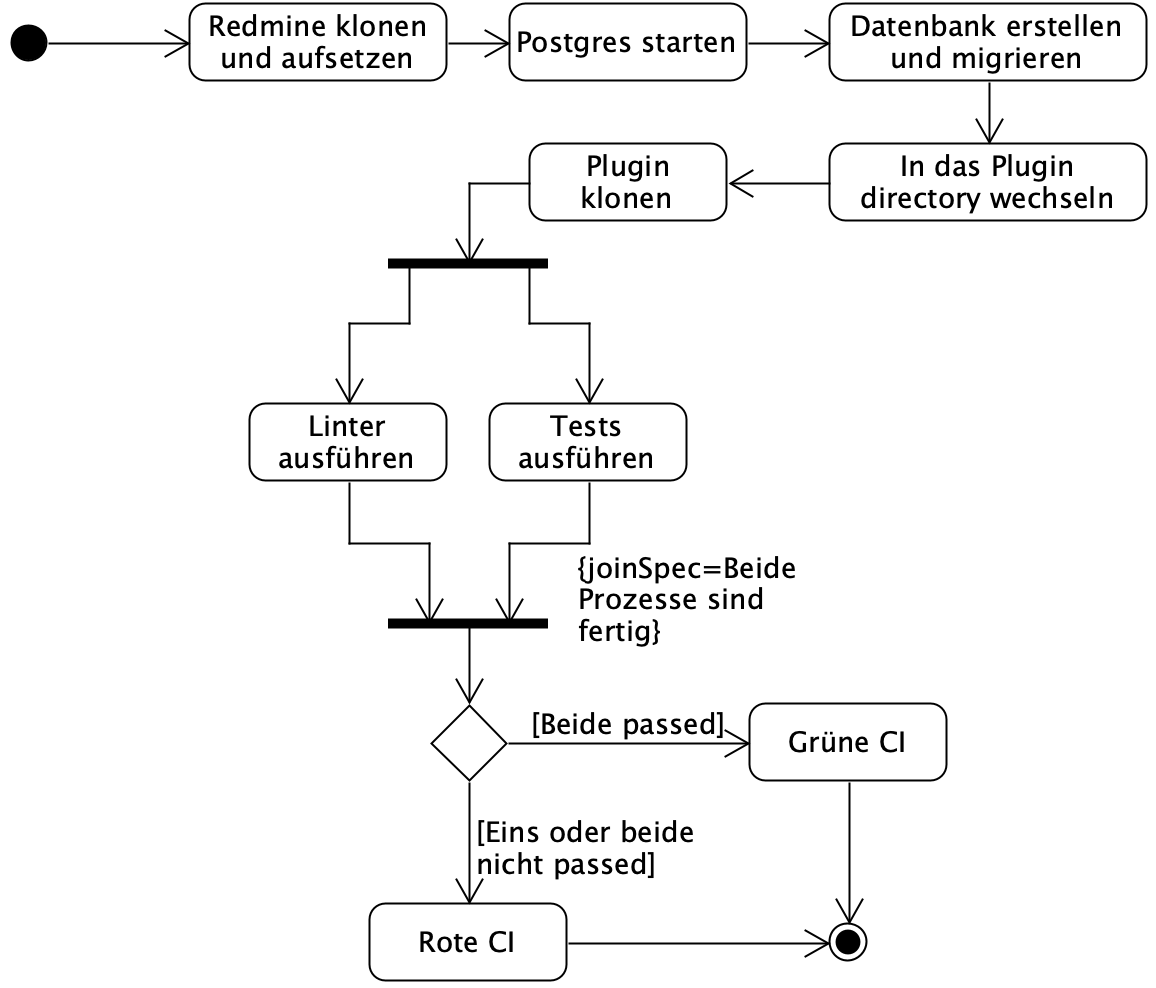
\includegraphics[width=0.8\textwidth]{images/activity/ci-cd.png}
    \label{fig:activity_ci_cd}
    \newline
  \end{center}
\end{minipage}

\begin{minipage}{\textwidth}
  Die oben beschriebene semaphore.yml Datei sieht dann so aus:
  \begin{codebox}[]
    \begin{minted}{yaml}
version: v1.0
name: Initial Pipeline
agent:
  machine:
    type: e1-standard-2
    os_image: ubuntu2004
blocks:
  - name: Checks
    task:
      jobs:
        - name: Tests
          commands:
            - bin/test
        - name: Linter
          commands:
            - bin/fastcheck
      prologue:
        commands:
          - 'git clone git@github.com:redmine/redmine.git'
          - cd redmine
          - cp config/configuration.yml.example config/configuration.yml
          - 'git clone git@github.com:aneshodza/redmine-postgres-database-yml.git'
          - cp redmine-postgres-database-yml/database.yml config/database.yml
          - rm -rf redmine-postgres-database-yml
          - bin/bundle install
          - yarn
          - sem-service start postgres --username="root" --password=""
          - 'bin/rails db:create'
          - 'bin/rails db:migrate'
          - cd plugins
          - checkout
          - cd ../../
          - bin/bundle install
          - cd plugins/gnosis
          - bin/setup
    \end{minted}
  \end{codebox}
  \textbf{Wichtig:} Auf Zeile 22 wird von einem Repository geklont. Das hat den Grund, dass das
  \bgmintinline{bash}{database.example.yml} nicht mit der MySQL Version von SemaphoreCI kompatibel ist. Das führt dazu,
  dass die Migrationen nicht durchlaufen können, wie in diesem StackOverflow issue beschrieben: \newline
  \url{https://stackoverflow.com/questions/63158705/rails-migration-mysql2error-specified-key-was-too-long-max-key-length-is-7}
  \newline
  Deswegen wird eine eigene Datenbank-Konfiguration verwendet.
\end{minipage}

\begin{minipage}{\textwidth}
  Nachdem das alles erledigt wurde, wird schnell ersichtlich, ob alles richtig ist oder nicht. In diesem Fall soll die CI
  grün sein: \newline
  \begin{center}
    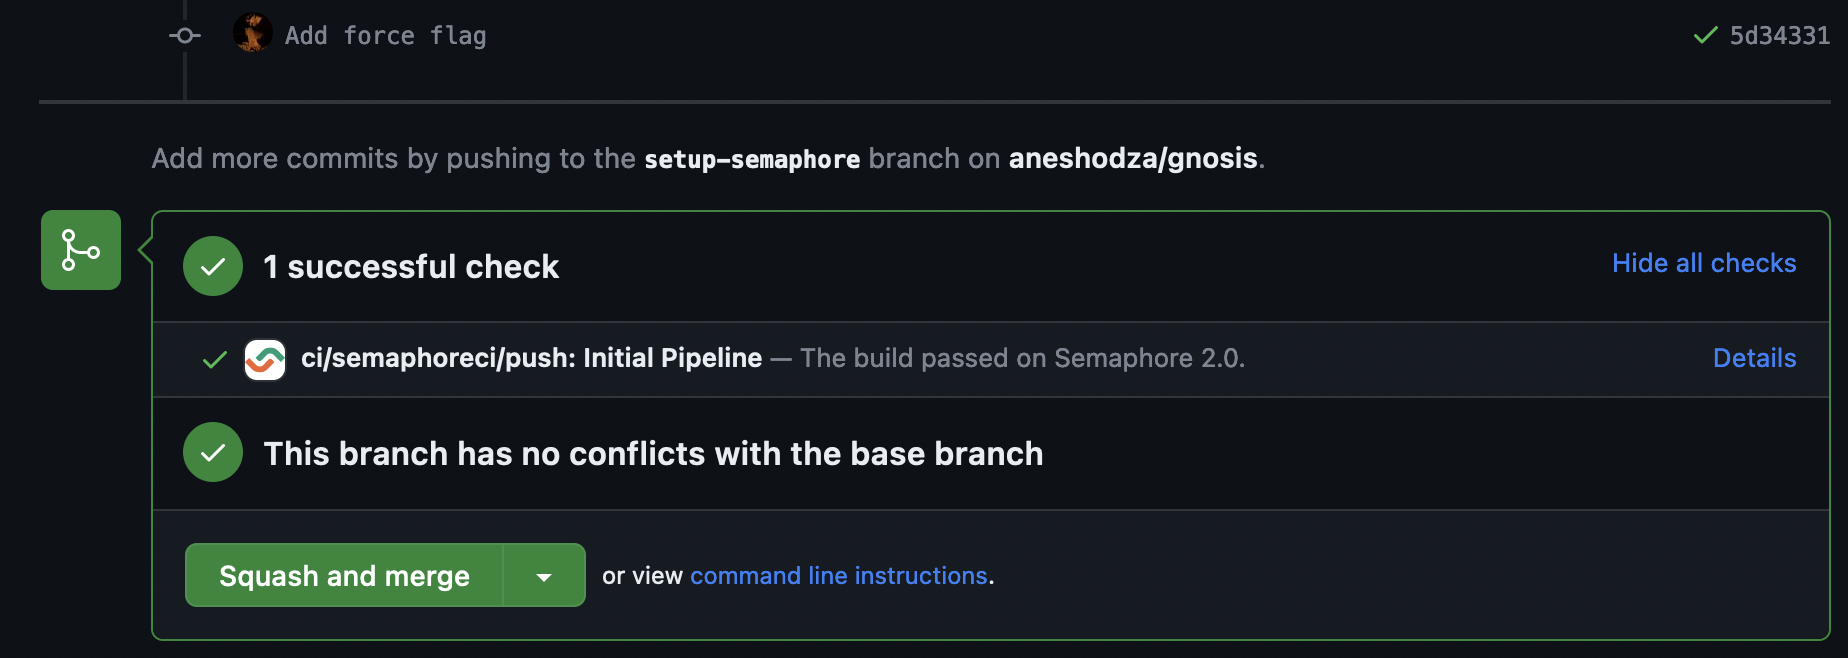
\includegraphics[width=0.8\textwidth]{images/misc/ci-passed.png}
    \label{fig:semaphore_ci_passed}
    \newline
  \end{center}
\end{minipage}

\begin{minipage}{\textwidth}
  \subsection{SimpleCov}
  Um die Test-Coverage zu messen, wird SimpleCov verwendet. SimpleCov ist ein Ruby Gem, welches die Test-Coverage misst und
  dann in einem HTML Report ausgibt. Ausserdem kann man eine minimale Test-Coverage definieren, welche beim Unterschreiten
  die Tests fehlschlagen lässt. \newline
  Die Implementation findet im test\_helper.rb statt und sieht wie folgt aus:
  \begin{codebox}[]
    \begin{minted}{ruby}
# frozen_string_literal: true

require 'simplecov'

SimpleCov.coverage_dir('plugins/gnosis/coverage')
SimpleCov.start do
  add_filter do |source_file|
    source_file.lines.count < 7
  end

  add_filter do |source_file|
    source_file.filename.exclude?('gnosis/app')
  end
end

SimpleCov.minimum_coverage 100

# Load the Redmine helper
require File.expand_path("#{File.dirname(__FILE__)}/../../../test/test_helper")
    \end{minted}
  \end{codebox}
  \textbf{Zu beachten:} Auf Zeile acht wird die mindeste Zeilenanzahl der Dateien auf 7 anstatt 5 gesetzt. Das hat den
  Grund, dass Rails Klassen meistens mit einem \bgmintinline{ruby}{# frozen_string_literal: true} gefolgt von einer
  leeren Zeile beginnen. Das führt dazu, dass Klassen mit vier Zeilen zu Dateien mit sechs Zeilen führen. \newline

  Wenn wir dann unser Plugin testen, gibt SimpleCov folgenden Report aus:
  \begin{codebox}
    \begin{minted}{bash}
Coverage report generated for Minitest to /Users/anes/c/redmine/plugins/gnosis/coverage. 3 / 3 LOC (100.0%) covered.
    \end{minted}
  \end{codebox}
\end{minipage}

\begin{minipage}{\textwidth}
  \section{Umsetzung der Datenstruktur}
  Da unter Kapitel \ref{sec:decide_erd} die Entscheidung getroffen wurde die \enquote{has many trough} Beziehung zu
  verwenden, wird diese auch implementiert. Das bedeutet, dass wir zwei Objekte erstellen müssen: 
  \bgmintinline{ruby}{PullRequest} und \bgmintinline{ruby}{Deployment}. Diese muss man mit dem Redmine CLI generieren,
  damit die neuen Objekte richtig mit den anderen Objekten von Redmine interagieren können. Für das Generieren unserer
  Objekte muss man folgende Befehle ausführen:
  \begin{codebox}[]
    \begin{minted}{bash}
rails generate redmine_plugin_model gnosis PullRequest 
rails generate redmine_plugin_model gnosis Deployment
rake redmine:plugins:migrate
    \end{minted}
  \end{codebox}
  \textbf{Wichtig:} Die Migrationen wurden noch mit den Attributen aus dem ERD befüllt. \newline
  Um dann die Associations nach Rails Standard zu machen, müssen wir unsere neuen Objekte wie folgt anpassen:
  \begin{codebox}[]
    \begin{minted}{ruby}
# app/models/pull_request.rb
class PullRequest < ApplicationRecord
  belongs_to :issue
  has_many :deployments, dependent: :destroy
end

# app/models/deployment.rb
class Deployment < ApplicationRecord
  belongs_to :pull_request
  has_one :issue, through: :pull_request
end

# app/models/gnosis_application_record.rb
class GnosisApplicationRecord < ActiveRecord::Base
  self.abstract_class = true
end
    \end{minted}
  \end{codebox}
\end{minipage}


  \chapter{Kontrollieren}

\section{Testprotokoll}
Dieser Abschnitt protokolliert das Testkonzept (siehe Kapitel \ref{sec:testkonzept}).
\subsection{Manuelle Tests}
\label{sec:manual-tests}
Die manuellen Tests wurden unter \ref{sec:manual-testing} vorgegeben. Hier werden die Ergebnisse
dokumentiert.
\begin{tabularx}{\textwidth}[H]{|c|X|X|}
    \hline
    \textbf{Nr.} & \textbf{Resultat} & \textbf{Datum und Uhrzeit} \\ \hline
    1 & Bestanden & 1. Juni 2023, 16:20 \\ \hline
    2 & Bestanden & 1. Juni 2023, 16:25 \\ \hline
    3 & Bestanden & 1. Juni 2023, 16:35 \\ \hline
    4 & Bestanden & 1. Juni 2023, 16:40 \\ \hline
\end{tabularx}

\subsection{Automatisierte Tests}
\label{sec:automated-tests}
Die automatisierten Tests wurden mit MiniTest und Capybara geschrieben, wie von Redmine selbst
vorgegeben. Auch das laufen lassen der Tests basiert auf dem vom Redmine vorgegebenen Rake Task. Um die
Tests laufen zu lassen, muss man \bgmintinline{bash}{rake redmine:plugins:test NAME=gnosis} im Terminal
ausführen. Dabei wird der Name des Plugins angegeben, damit nur die Tests für dieses Plugin laufen. Im
\bgmintinline{bash}{bin} Verzeichnis befindet sich eine \bgmintinline{bash}{bin/test} Datei, welche
diesen Rake Task ausführt und den Output schön formatiert.
Der Output sieht dann ungefähr so aus:
\begin{center}
    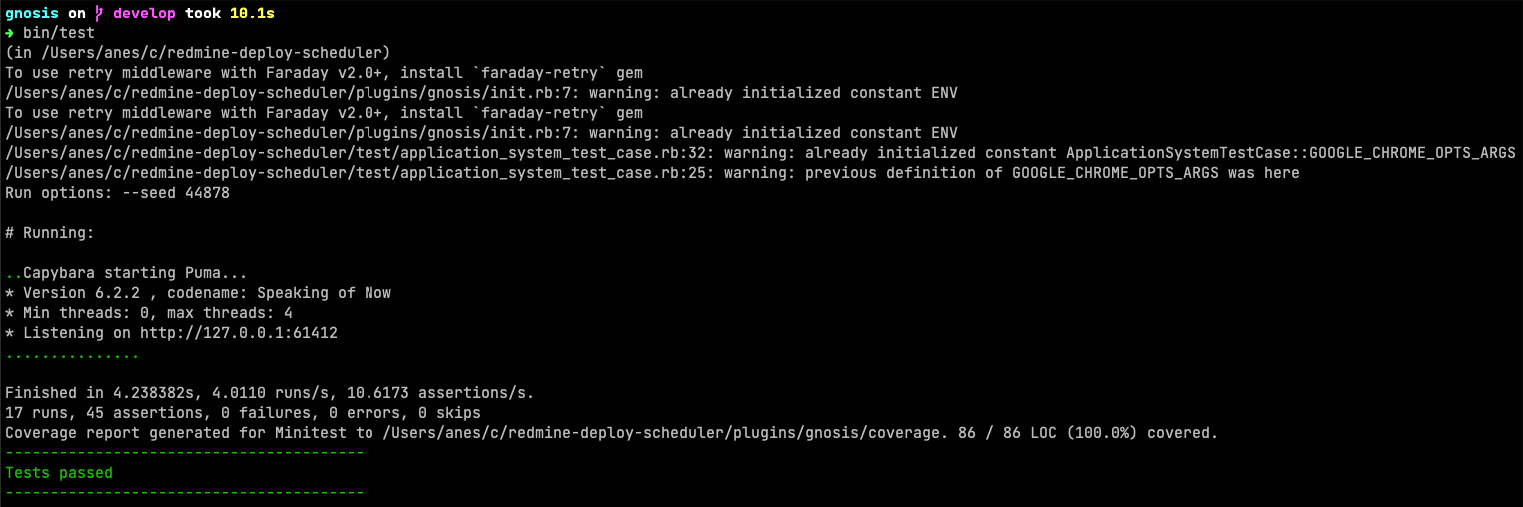
\includegraphics[width=0.75\textwidth]{images/misc/simplecov_terminal_output.png}
    \label{fig:simplecov_terminal_output}
\end{center}
SimpleCov generiert auch eine HTML Datei, in welcher die Coverage jeder Zeile genau markiert ist in
rot oder grün, je nachdem, ob es getestet wurde oder nicht. So sieht diese Datei in diesem Fall aus:
\begin{center}
    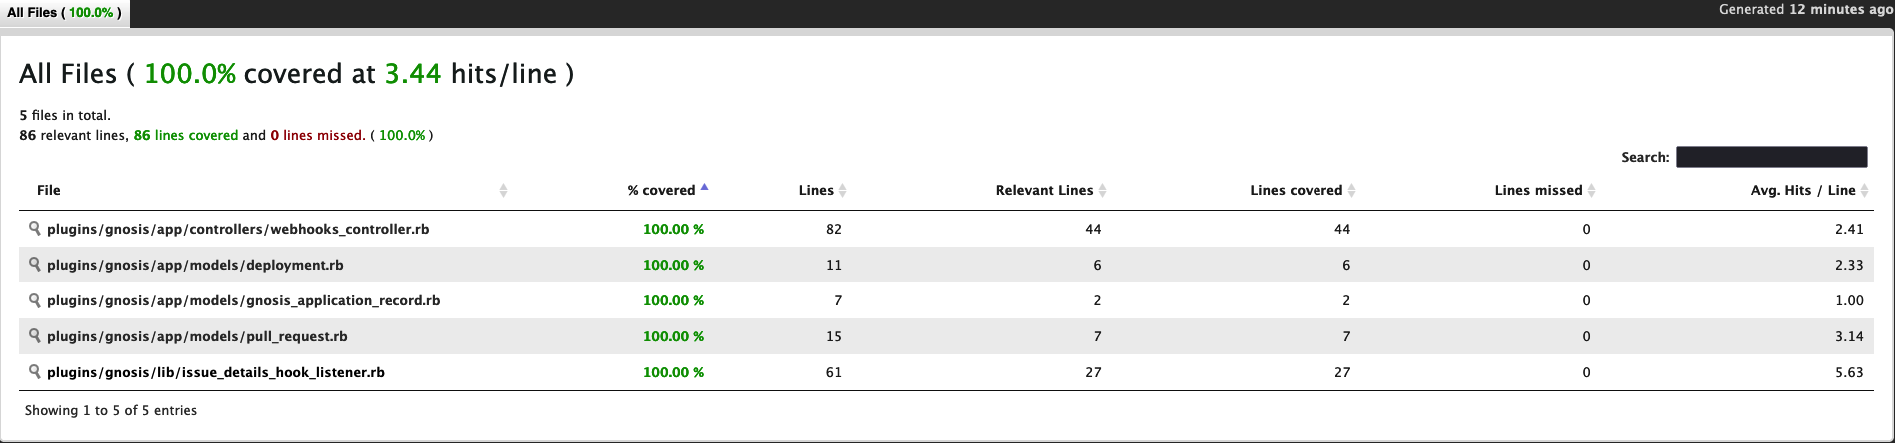
\includegraphics[width=0.75\textwidth]{images/misc/simplecov_html.png}
    \label{fig:simplecov_html_output}
\end{center}

\subsubsection{Verscheidene Testarten}
Die Tests befinden sich im \bgmintinline{bash}{test} Verzeichnis. Dort werden diese in verschiedene
Gruppen aufgeteilt, basierend auf der Testart. Die Gruppen sind:
\begin{itemize}
    \item \bgmintinline{bash}{functional} - Funktionale Tests senden Anfragen an die Controller.
    \item \bgmintinline{bash}{unit} - Unittests, welche die einzelnen Klassen und dessen Methoden
    testen.
    \item \bgmintinline{bash}{system} - System Tests klicken sich mit Capybara durch die UI des
    Plugins und testen so die Funktionalität.
\end{itemize}
Die funktionalen Tests wurden für das Testen des \bgmintinline{ruby}{class WebhooksController}
genutzt. Sie schicken Anfragen an den Controller und desssen Funktionen und testen so, ob die richtigen
Objekte basierend auf dem erstellt werden. \newline
Die Unittests wurden für das Testen der \bgmintinline{ruby}{class Deployment} und 
\bgmintinline{ruby}{class PullRequest} genutzt. Sie testen die einzelnen Methoden dieser Klassen und
prüfen, ob die Objekte richtig manipuliert werden. \newline
Die Systemtests werden für das Testen der UI genutzt. Mithilfe von Capybara wird ein Headless Browser
gestartet, welcher sich durch die UI klickt und so die Funktionalität testet.
\subsection{Style Tests}
Damit der Code \enquote{Clean Code} bleibt, werden Linter verwendet. Diese überprüfen den Code auf Stilfehler,
Sicherheitslücken und andere Fehler. \newline
Da dieses Projekt nur aus Ruby Code besteht, wurde Rubocop in Zusammenarbeit mit Brakeman verwendet. Rubocop
ist dafür zuständig Bugs und Stilfehler zu finden, während Brakeman Sicherheitslücken findet. Diese beiden
Prozesse wurden auch in der CI Pipeline eingebaut, damit der Code immer sauber bleibt:
\begin{center}
    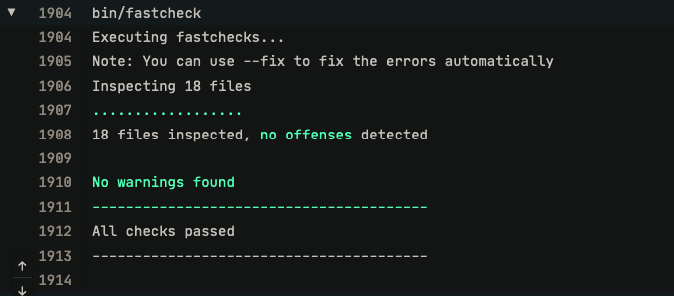
\includegraphics[width=0.75\textwidth]{images/misc/stylecheck_ci.png}
    \label{fig:ci_pipeline}
\end{center}

\section{Versionierung}
In diesem Kapitel wird die Versionierung von Dokumentation sowie Programmcode beschrieben.
\subsection{Dokumentation}
Die Dokumentation wird mit LaTeX geschrieben und deswegen auch mit Git auf GitHub versioniert. Das
Repository kann unter \url{https://github.com/aneshodza/ipa-documentation} gefunden werden.
\subsubsection{Git-Flow}
Die Versionierung wird nach dem \enquote{Git-Flow} Prinzip gemacht. Das heisst: Es gibt einen main sowie
develop Branch. Der main Branch wird nur bei Releases geändert. Der develop Branch wird für die normale
Entwicklung genutzt. Für jedes neue Kapitel wird ein Feature Branch erstellt.
\subsubsection{Releases}
Am Ende jedes Tages wird ein \enquote{Release} erstellt. Damit ist nicht der main release gemeint, da dieser
nur am Ende des Projekts erstellt wird. Diese Releases finden per Git Tag statt. Dabei wird der letzte
Commit eines Tages mit einem Tag markiert. Das sieht wie folgt aus:
\begin{center}
    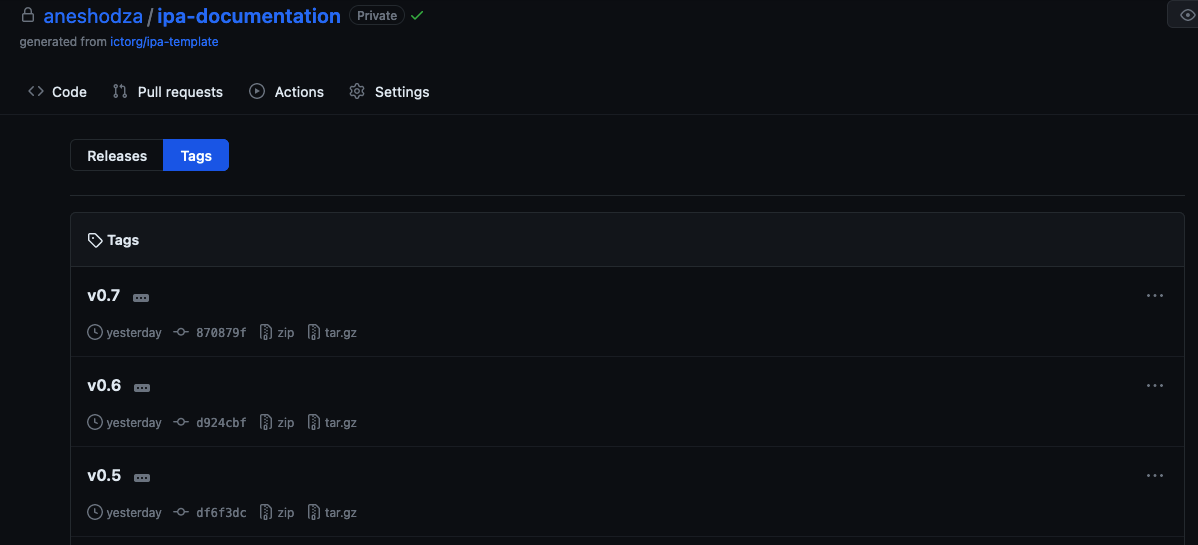
\includegraphics[width=0.75\textwidth]{images/misc/git_tag.png}
    \label{fig:git_tag}
\end{center}

\subsection{Programm}
Der Programmcode wird auch mit Git auf GitHub versioniert. Das Repository kann unter
\url{https://github.com/aneshodza/gnosis} gefunden werden.
\subsubsection{Git-Flow}
Die Versionierung dieses Repositorys wird auch nach dem \enquote{Git-Flow} Prinzip gemacht. Dabei wird
speziell darauf geachtet, dass alle Commit-Messages auf Englisch, imperativ und in der Gegenwartsform
geschrieben sind: 
\begin{center}
    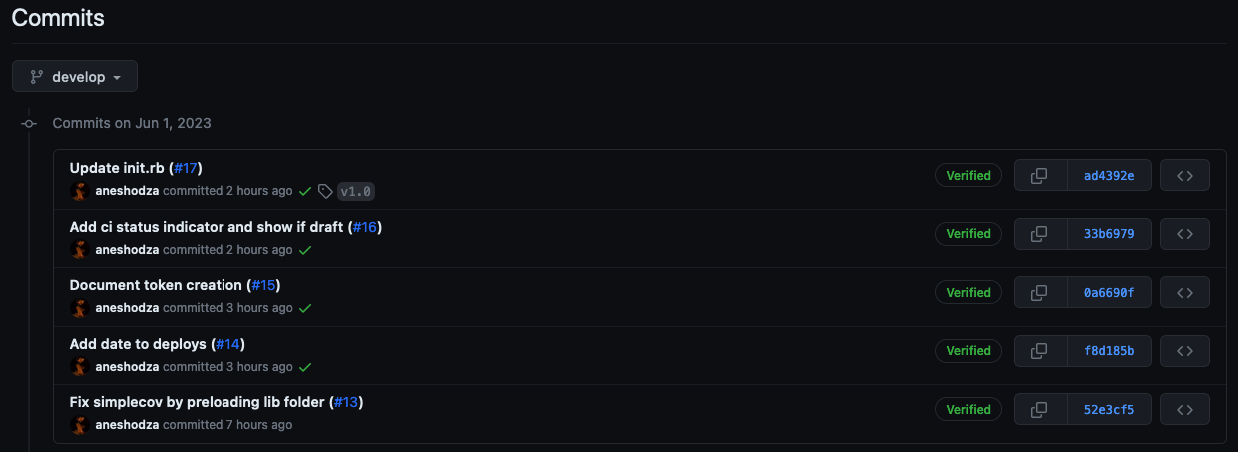
\includegraphics[width=0.75\textwidth]{images/misc/git_commit_message.png}
    \label{fig:git_commit_message}
\end{center}
\subsubsection{Selbstkritische Pull Request Reviews}
Bei grösseren Pull Requests wurde ein selbstkritisches Review gemacht. Dabei wurde der Code nochmals
durchgegangen und überprüft, ob grobe Fehler zu finden sind:
\begin{center}
    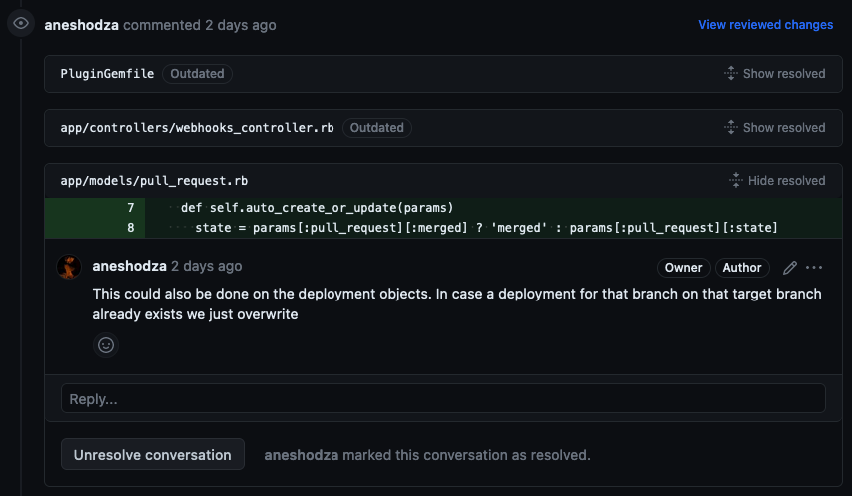
\includegraphics[width=0.75\textwidth]{images/misc/git_pr_review.png}
    \label{fig:git_pr_review}
\end{center}
\subsubsection{Arbeitspakete mit \gls{grün}er CI}
Die Pull Requests entsprechen meistens geplanten Arbeitspaketen und wurden deswegen auch so benannt. Es hat
aber auch einige Pull Requests, welche kein AP waren, da Dinge wie Bugfixes oder Refactorings nicht geplant
werden können. \newline
Dabei wurde auch darauf geachtet, dass der neuste Commit jeder Pull Request grün ist.

\section{Kopplung vom Hauptprogramm}


  \chapter{Auswerten}
In diesem Kapitel wird die PA kritisch ausgewertet. Dabei wird auf die Erfüllung der Anforderungen eingegangen
und die Probleme, welche während der PA aufgetreten sind, beschrieben.

\section{Erfüllungsgrad der Anforderungen}
Das erhaltene Produkt dieser PA hat zwei Teile: Die Dokumentation und das Programm.
\subsection{Dokumentation}
Die Dokumentation stammt von einem Template \cite{Buhler_ipa-template_2022} ab, welches in LaTeX geschrieben
wurde: Eine ganze \enquote{Programmiersprache}, welche sich sehr gut für Dokumentationen eignet. Dinge wie der
Glossar oder das Abbildungsverzeichnis werden von LaTeX automatisch generiert. \newline
Dazu wurde auch sehr viel Wert auf das Einhalten des Kriterienkatalogs gelegt, weshalb die Dokumentation auch
sehr vollständig sein.
\subsection{Programm}
Das Programm ist ein, komplett von Redmine abgekoppeltes, Plugin. Es wurde mit ERB und Ruby geschrieben, während
die (mit 100\% coverage) Tests mit MiniTest geschrieben wurden. Auch hier werden alle Kriterien erfüllt, da die
Anforderungen als \enquote{Leitfaden} genutzt wurden. Mit einer guten Planung für die Umsetzung ging auch die
Umsetzung sehr schnell. \newline
Was nicht gelungen ist, ist das aktive Polling zu vermeiden. Das heisst, dass das Plugin nach einer SemaphoreCI
Request zu GitHub geht und diesen Dienst nach einer Commit History fragt. Dies wird unter Kapitel
\ref{sec:why_active_polling} genauer beschrieben.

\section{Reflexion}
\subsection{Probleme}
Da diese PA ein Redmine Plugin schreiben musste, wurde folgendes Problem sehr offensichtlich: Die Arbeit ist
sehr Nische, was bedeutet, dass die Dokumentation mehr oder weniger die einzige Quelle ist
\cite{redmine_plugin_tutorial}. Falls Probleme auftreten, welche von der offiziellen Dokumentation nicht
abgedeckt sind, muss man wahrscheinlich einfach selber herumprobieren. Das war auch der Fall beim SimpleCov
Setup. Für den spezifischen Fall (mit dem Redmine Framework rundherum) gibt es keine Dokumentation, GitHub
Issues oder andere Quellen im Internet. \newline
Das führte dazu, dass für das Programm sehr viel Zeit eingeplant wurde, welche am Schluss doch nicht nötig war.
\subsection{Erfolge}
Der Vorteil des oben genannten Problems war, dass die mangelnde Dokumentation das Implementieren nur noch
spannender machte. Anstatt wie für alles bisher eine Dokumentation und hundert Frameworks zu nutzen, welche einem
die ganze Arbeit abnehmen, musste selbst viel erforscht werden. Wenn etwas ging, gab es immer sehr erfüllende
Siegesmomente. \newline
Ausserhalb des Programms wurde diese IPA mit LaTeX geschrieben. Das war eine sehr gute Wahl, da sich diese
Arbeit gut dafür eignete passiv noch einen Grundkurs in LaTeX zu absolvieren.

\section{Persönliche Bilanz}
Ich fand diese PA eine meiner spannendsten Arbeiten bisher. Das lag vor allem daran, dass die Dokumentation sehr
technisch und ausführlich war. Mir wurde aber im Verlauf der Arbeit klar, dass eine agile Projektplanung für
Software besser ist. Während dem Arbeiten merkte ich oft, dass es etwas zu tun gab, was nicht im Zeitplan oder
als Arbeitspaket aufgelistet war. Das führte zu einem ungenauen Zeitplan und vielen Einträgen unter
\enquote{Puffer}.

\section{Mögliche Verbesserungen/Erweiterungen}
Das Programm wurde unter einem sehr engen Zeitplan entwickelt. Das führte dazu, dass das Programm an bestimmten
Orten gut erweiterbar ist. Einige dieser Ideen werden hier aufgelistet:
\subsection{Eigene Konventionen}
Die erste Idee war, dass der Nutzer die Konventionen selbst entscheiden kann. Es gibt in Redmine Plugins die
Möglichkeit, dass der Nutzer das Plugin einstellen kann. Das könnte man mit dem Regex für das Finden von Issue
IDs machen.
\subsection{Mehrere CI Dienste}
Das Programm könnte auch so ausgebaut werden, dass es mehrere CI Dienste unterstützt. Das wäre wichtig bei
grossen Diensten, wie zum Beispiel TravisCI.


  % see B6.6
  % create a phantom toc entry for the index/glossary table
  \clearpage\phantomsection\addcontentsline{toc}{part}{Glossar}

  % generate glossary
  \printnoidxglossary[title={Glossar}]

  % create a phantom toc entry for the figures table
  \clearpage\phantomsection\addcontentsline{toc}{part}{Abbildungsverzeichnis}

  % generate figures table
  \listoffigures

  % create a phantom toc entry for the literature table
  \clearpage\phantomsection\addcontentsline{toc}{part}{Literaturverzeichnis}

  % generate bibliography
  \printbibliography[title=Literaturverzeichnis]

  % defines the beginning of the appendix
  \appendix

  % create a phantom toc entry for "Projekt"
  \clearpage\phantomsection\addcontentsline{toc}{part}{Anhang}

  % see B6.1b
\chapter{Quellcode}
In diesem Kapitel wird der Quellcode angehängt. Das Verzeichnis jeder Datei ist als Kommentar am Anfang
der Datei zu finden. \newline
\textbf{Wichtig:} Dieser Quellcode ist nicht vollständig.
Er beinhaltet nur selbst geschriebenen Code. Der Generierte Boilerplate vom Redmine CLI wurde nicht
hinzugefügt. Der Code ist auf GitHub zu finden: \url{https://github.com/aneshodza/gnosis}.


\end{document}
